\documentclass[11pt]{article}
\title{Laporan Tugas Basisdata II}
\author{Hanif Amrullah / 1184020}
\usepackage{graphicx}


\begin{document}
\maketitle

\section{Langkah-Langkah Membuat Aplikasi dengan Oracle}
Berikut langkah-langkah membuat aplikasi apex.
\begin{enumerate}

\item 
Kunjungi website oracle apex dan klik sign in
\begin{figure}[h]
\centerline {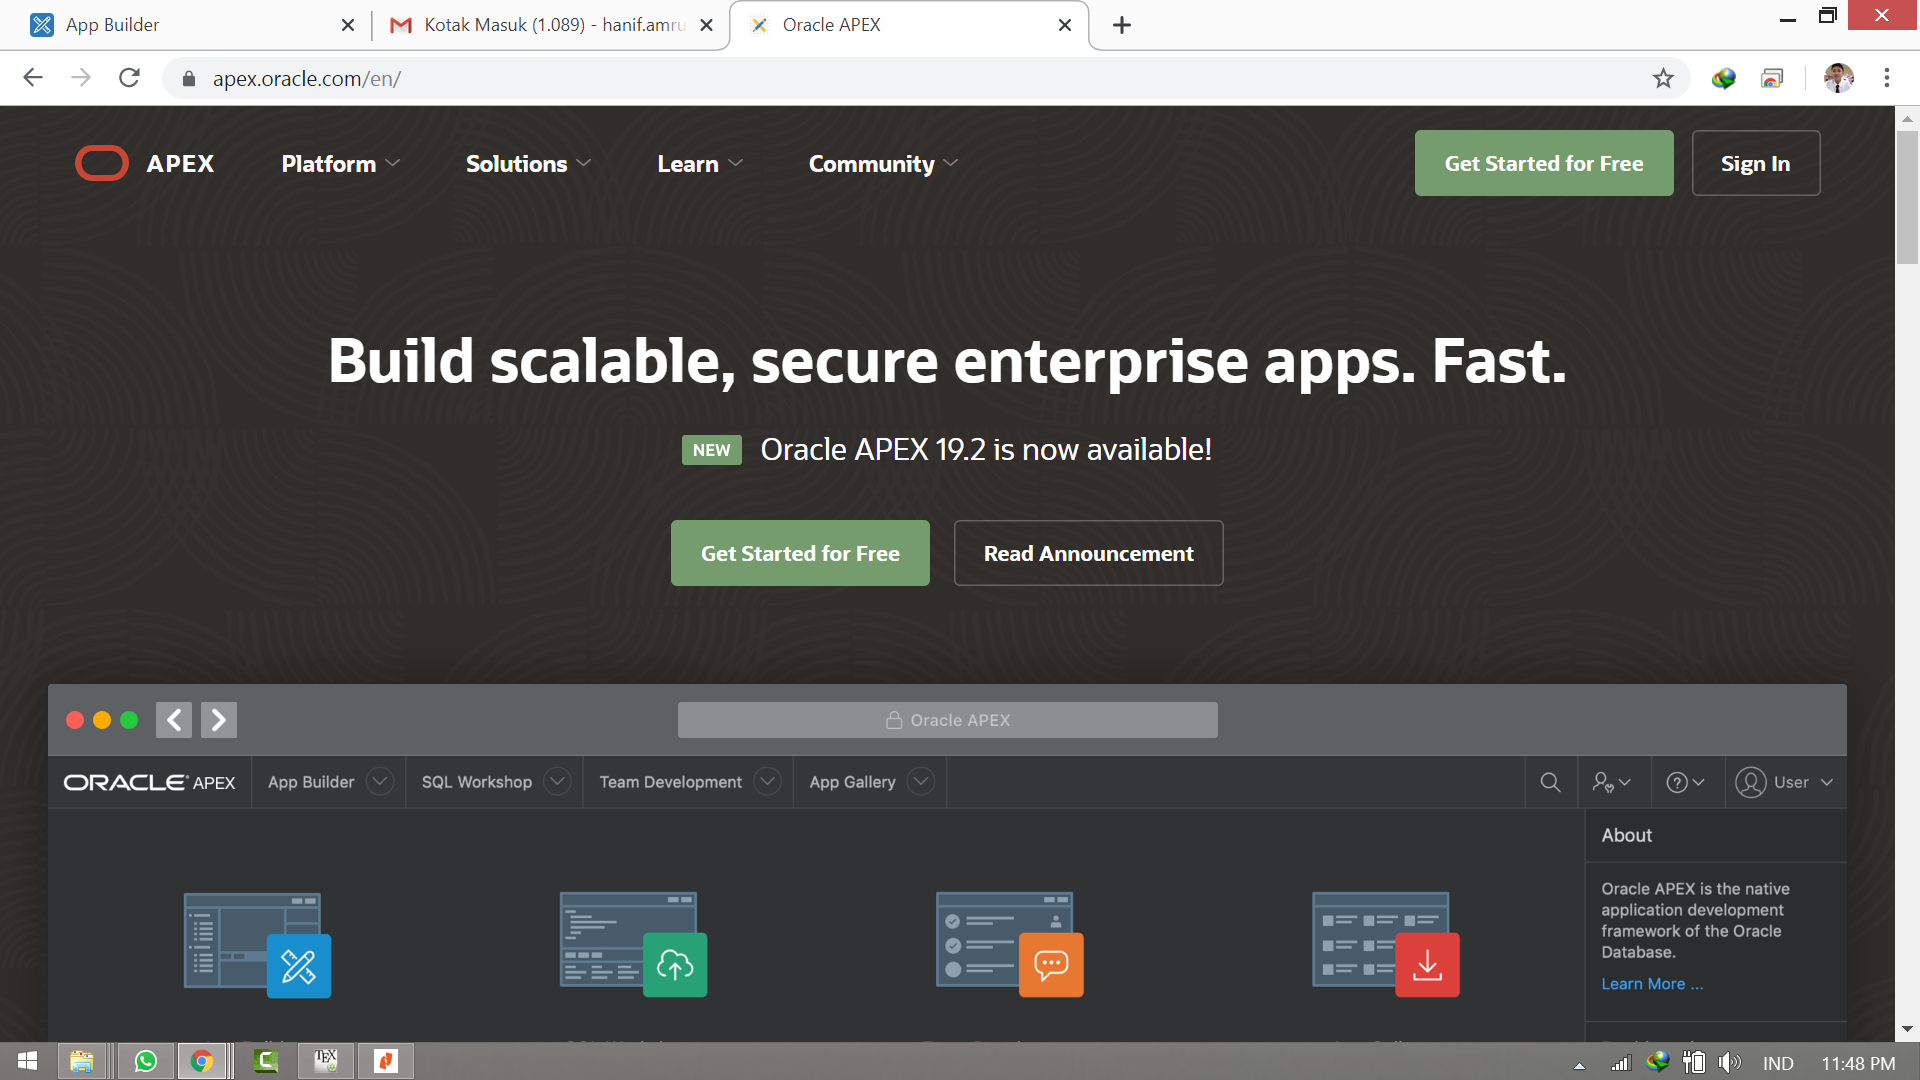
\includegraphics[scale=0.1]{img/web.png}}
\caption{}
\label{langkah1}
\end{figure}

\item isi WorkSpace,Username, Passwoard
\begin{figure}
        \centerline{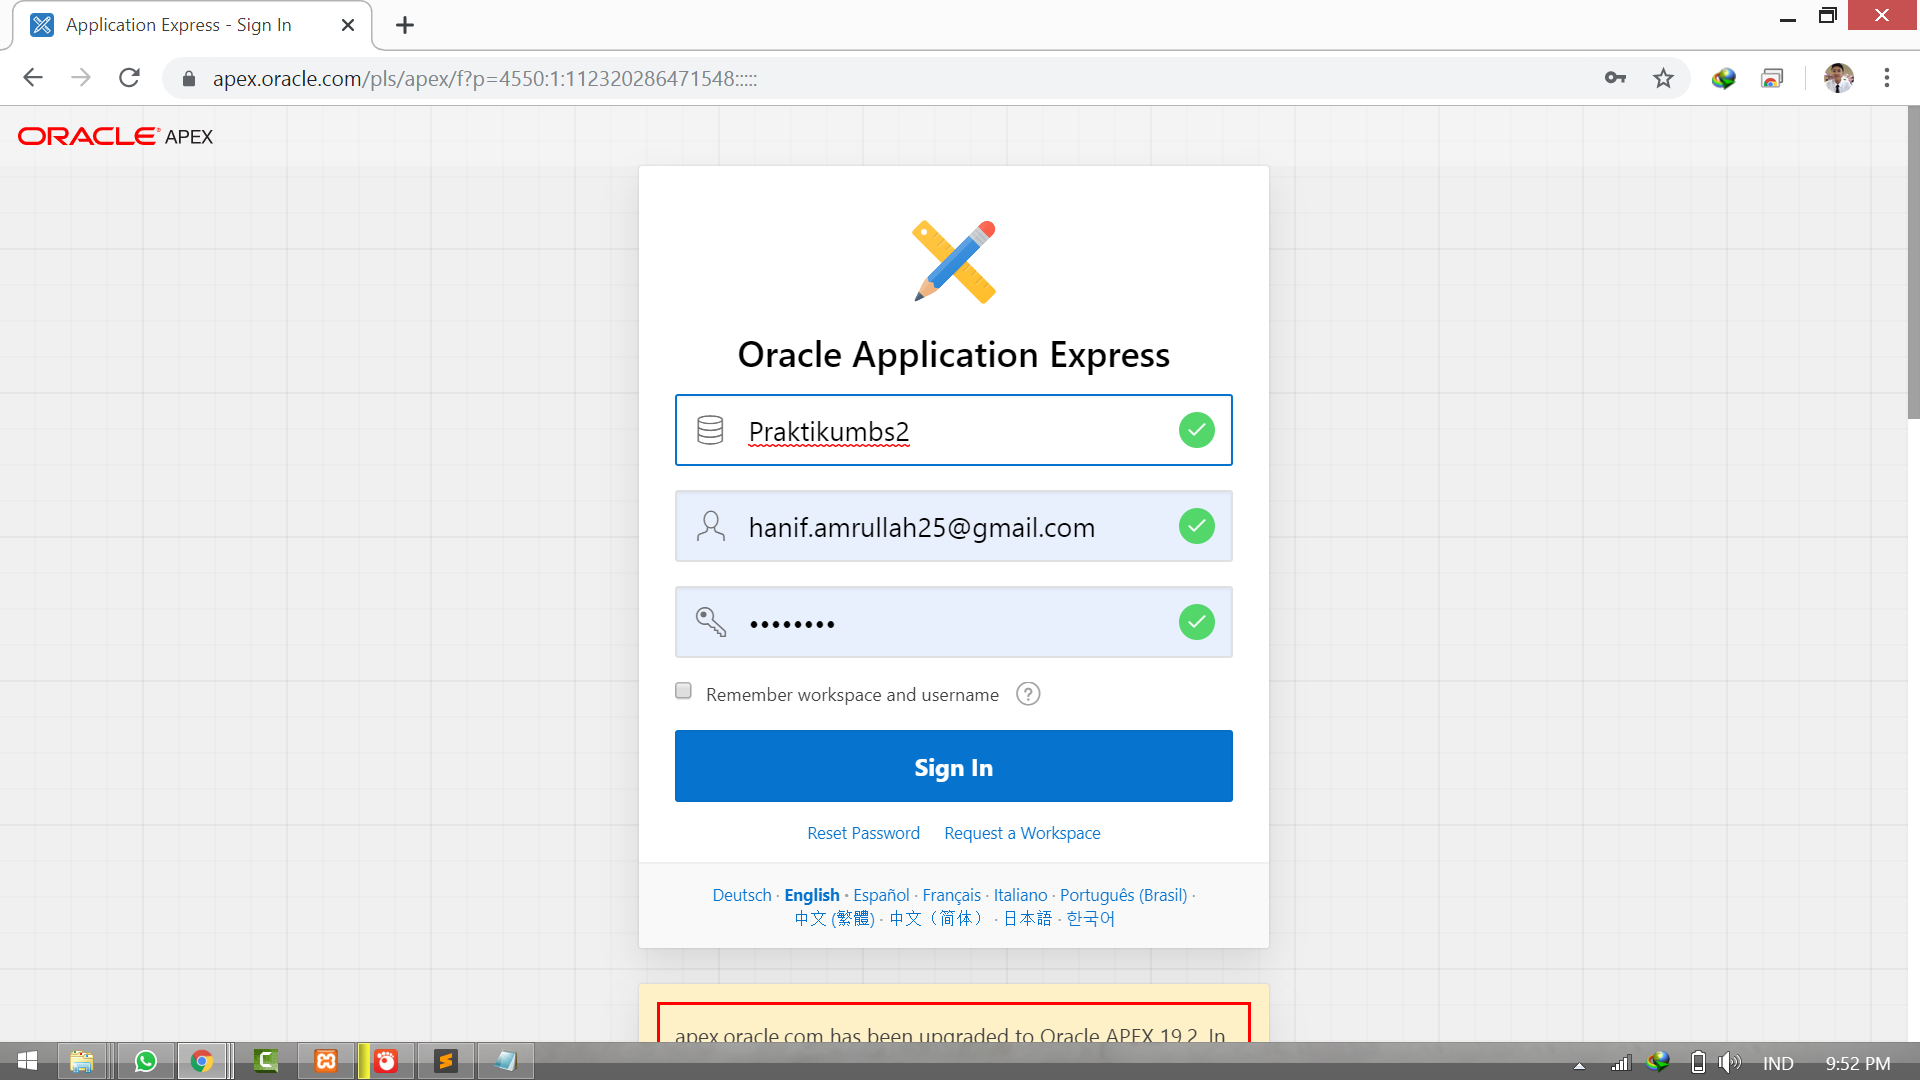
\includegraphics[scale=0.1]{img/1login.png}}
        \caption{}
		\label{langkah2}
\end{figure}

\item klik AppBuilder
\begin{figure}
        \centerline{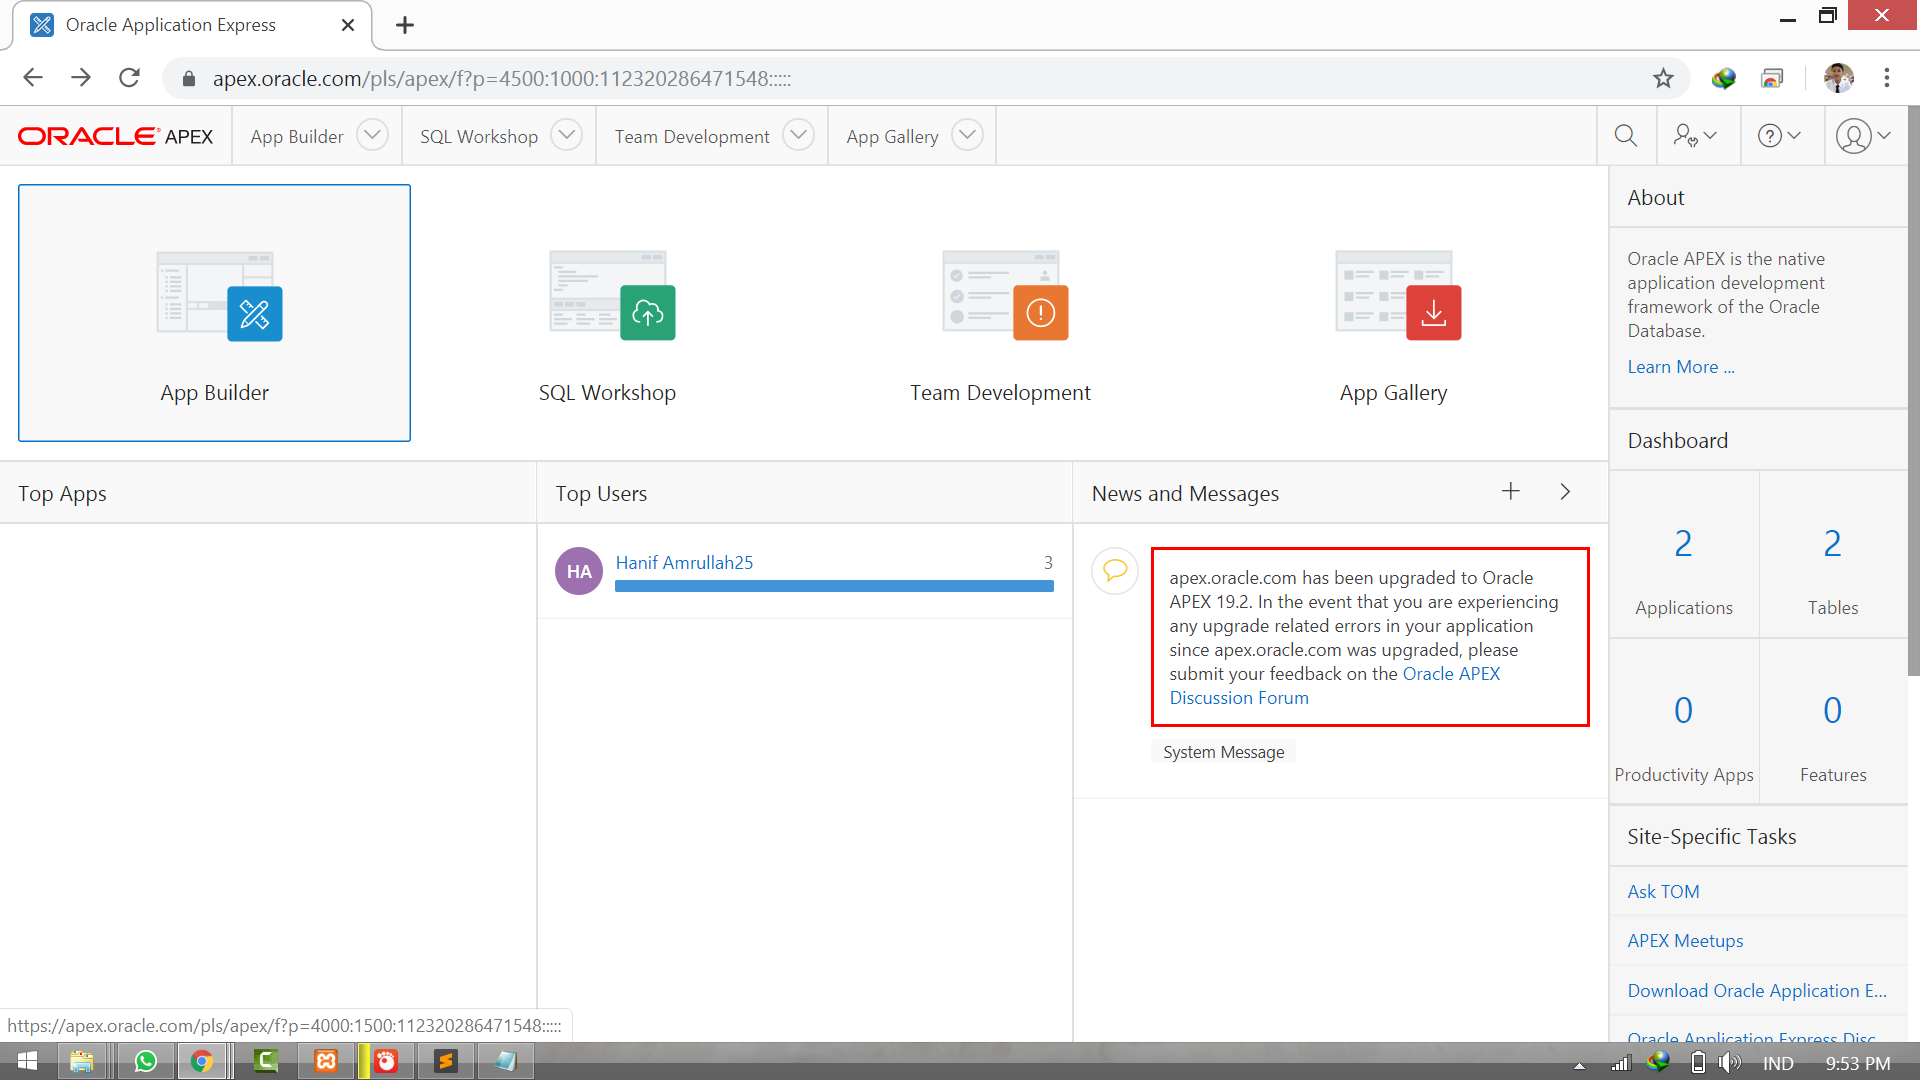
\includegraphics[scale=0.1]{img/2appbuilder.png}}
        \caption{}
		\label{langkah3}
\end{figure}

\item klik Create
\begin{figure}
        \centerline{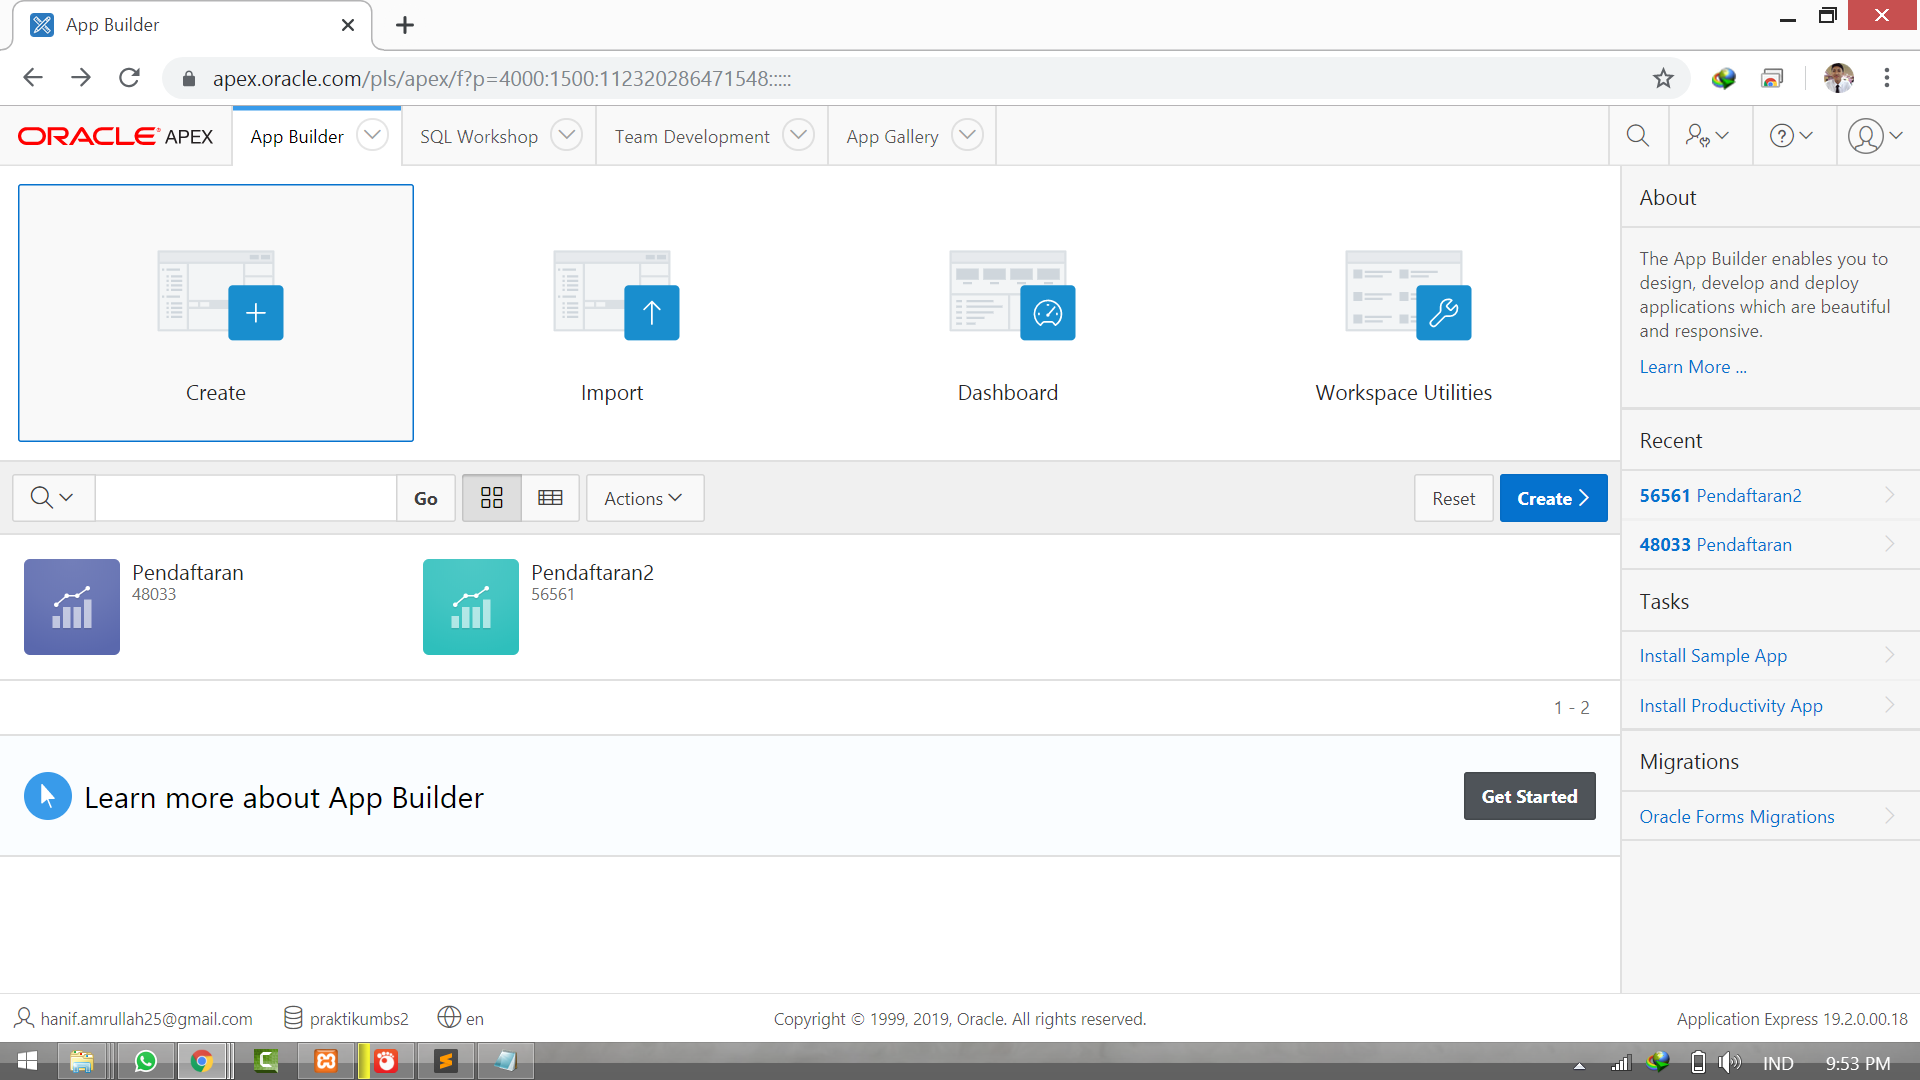
\includegraphics[scale=0.1]{img/3create.png}}
        \caption{}
		\label{langkah4}
\end{figure}

\item klik Form A File
\begin{figure}
        \centerline{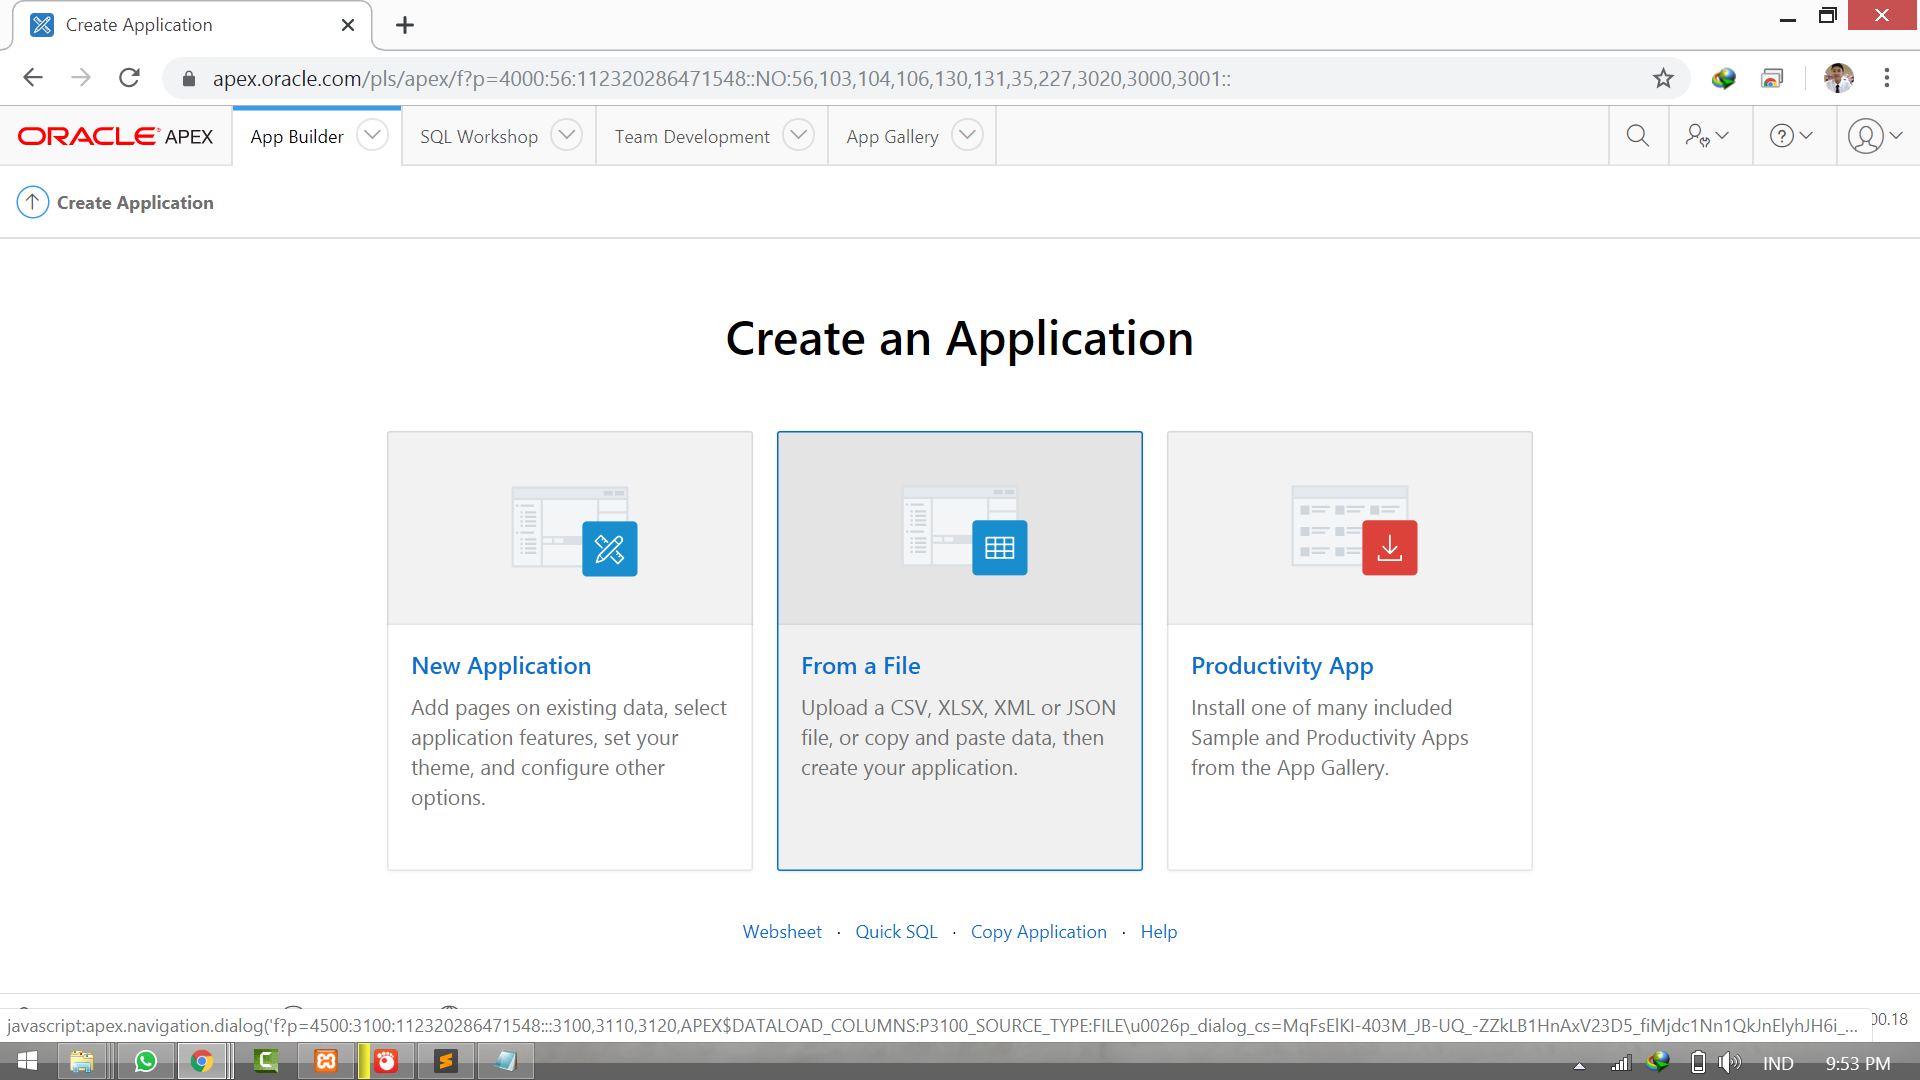
\includegraphics[scale=0.1]{img/4formfile.png}}
        \caption{}
		\label{langkah5}
\end{figure}

\item ikuti
\begin{figure}
        \centerline{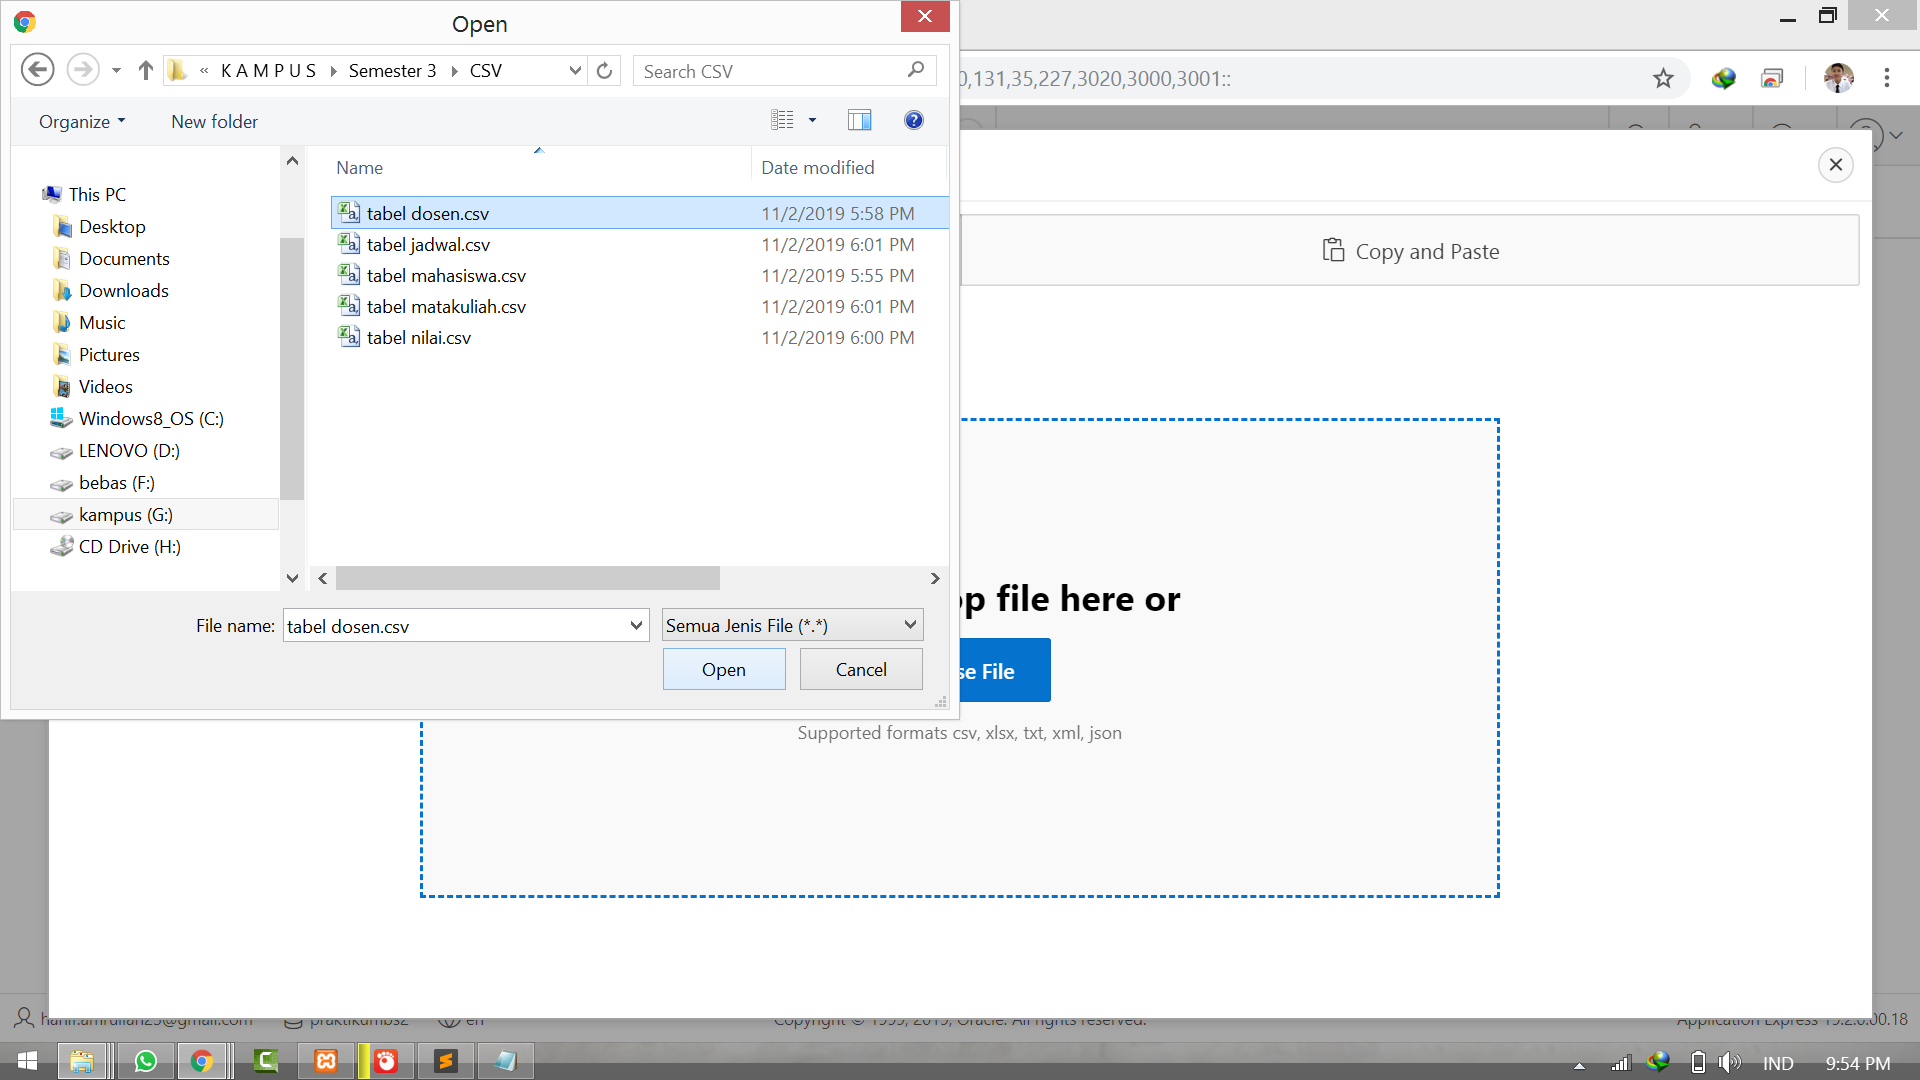
\includegraphics[scale=0.1]{img/5DragTabel.png}}
        \caption{}
		\label{langkah6}
\end{figure}

\item ikuti
\begin{figure}
        \centerline{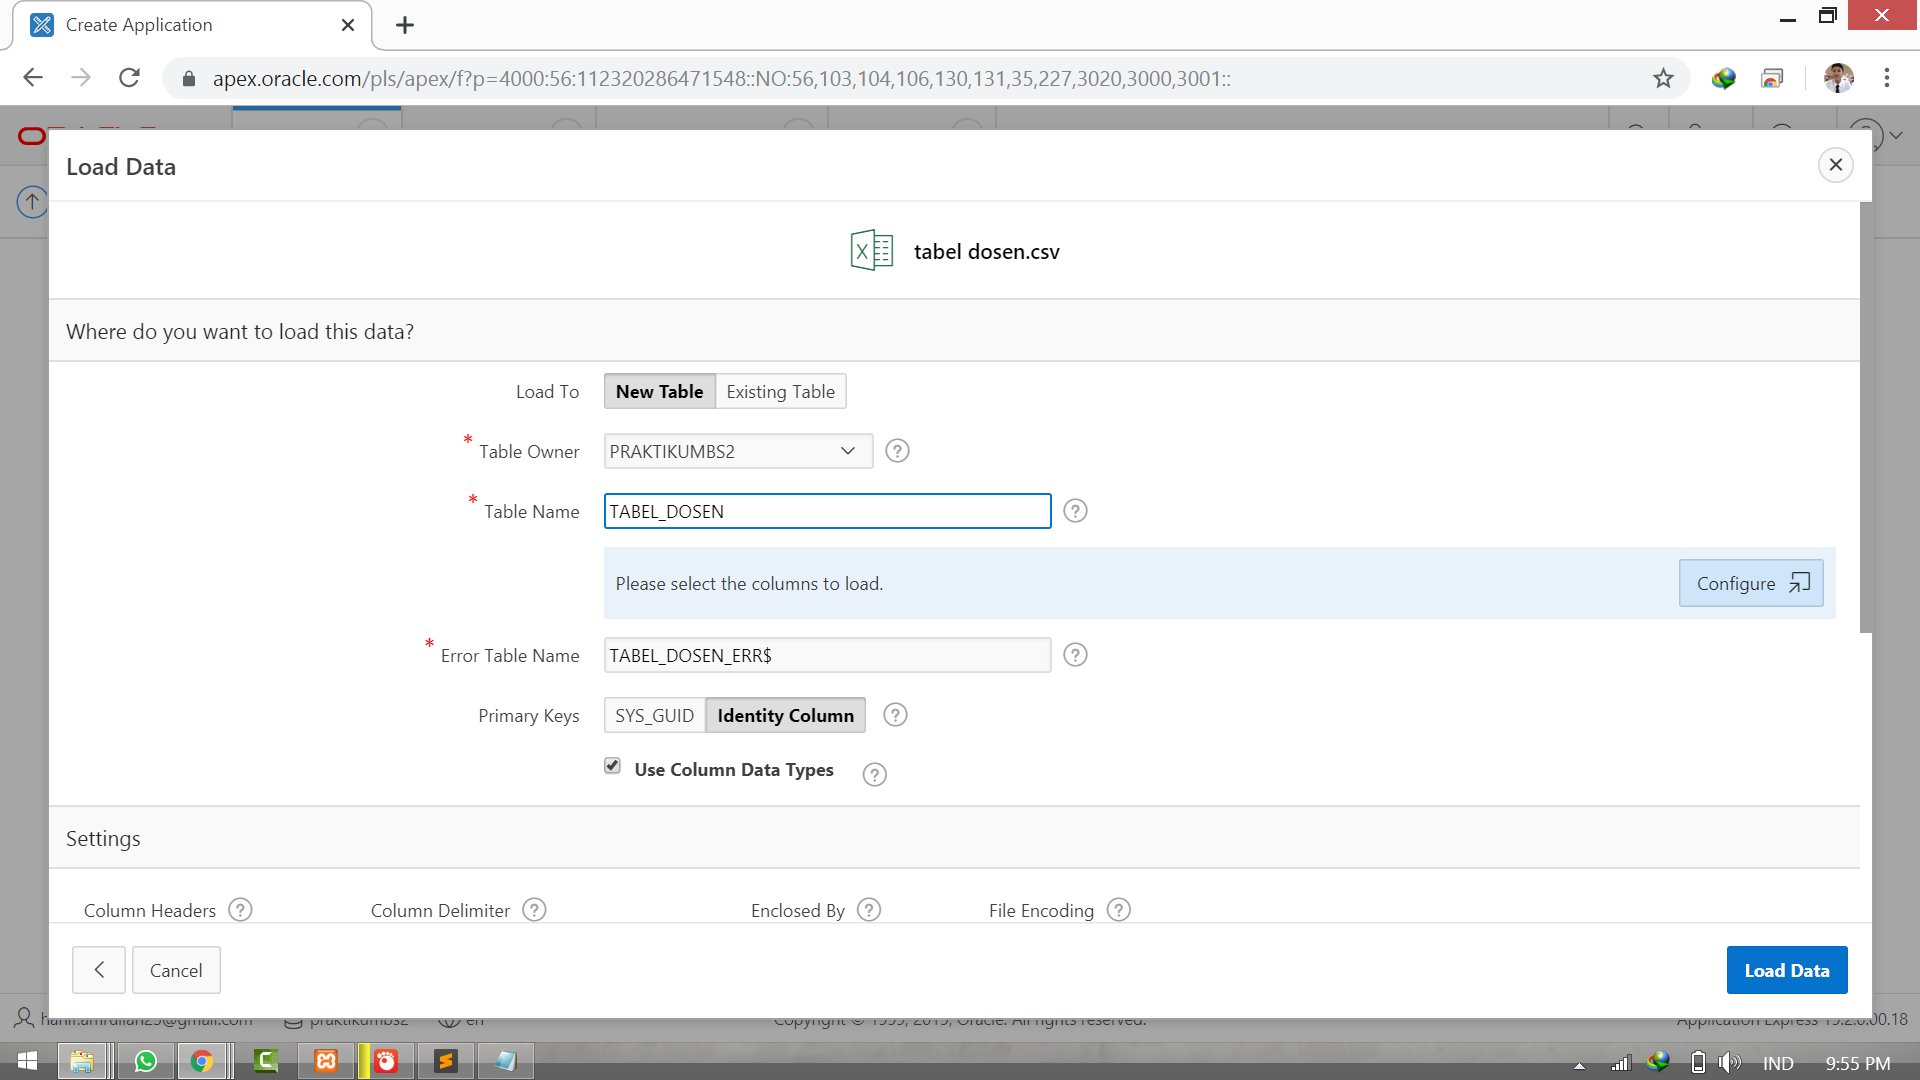
\includegraphics[scale=0.1]{img/6IsiNamaTabel.png}}
        \caption{}
		\label{langkah7}
\end{figure}

\item ikuti
\begin{figure}
        \centerline{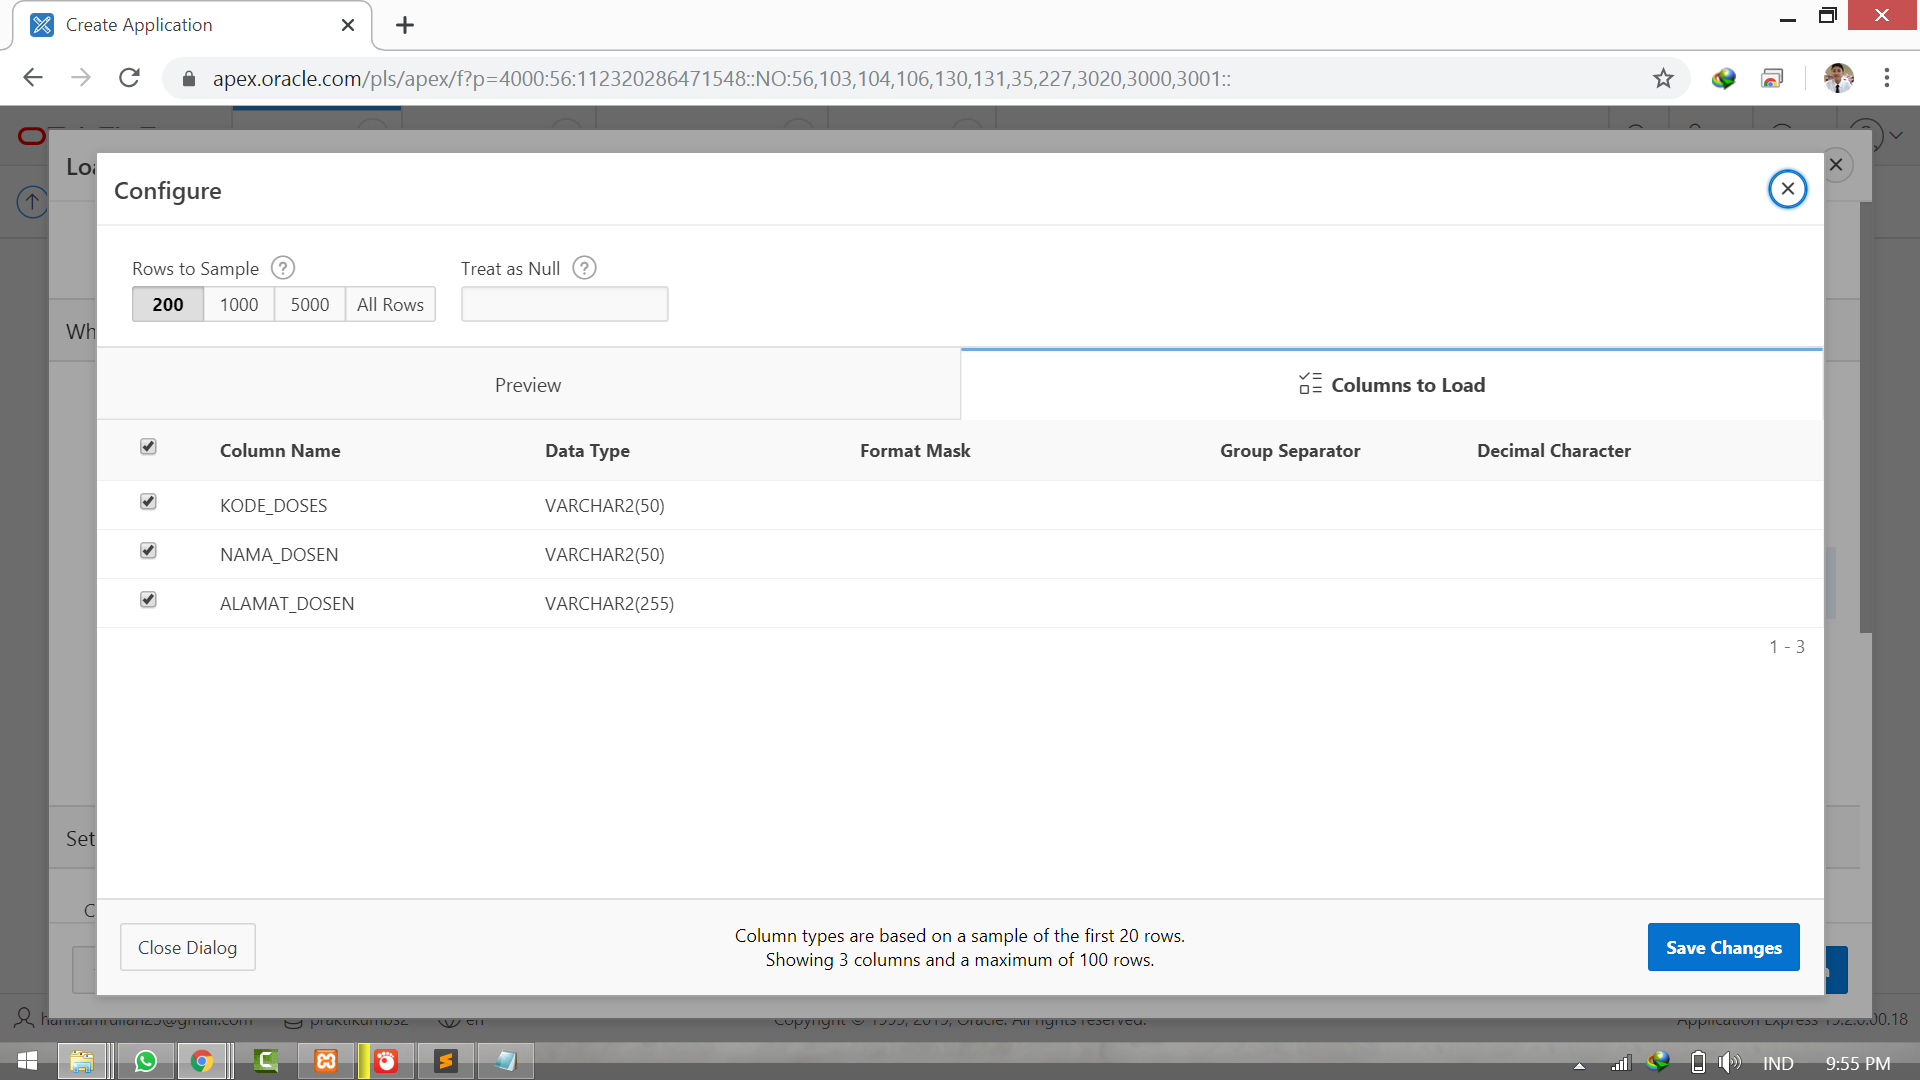
\includegraphics[scale=0.1]{img/7ConfigTabel.png}}
        \caption{}
		\label{langkah8}
\end{figure}

\item ikuti
\begin{figure}
        \centerline{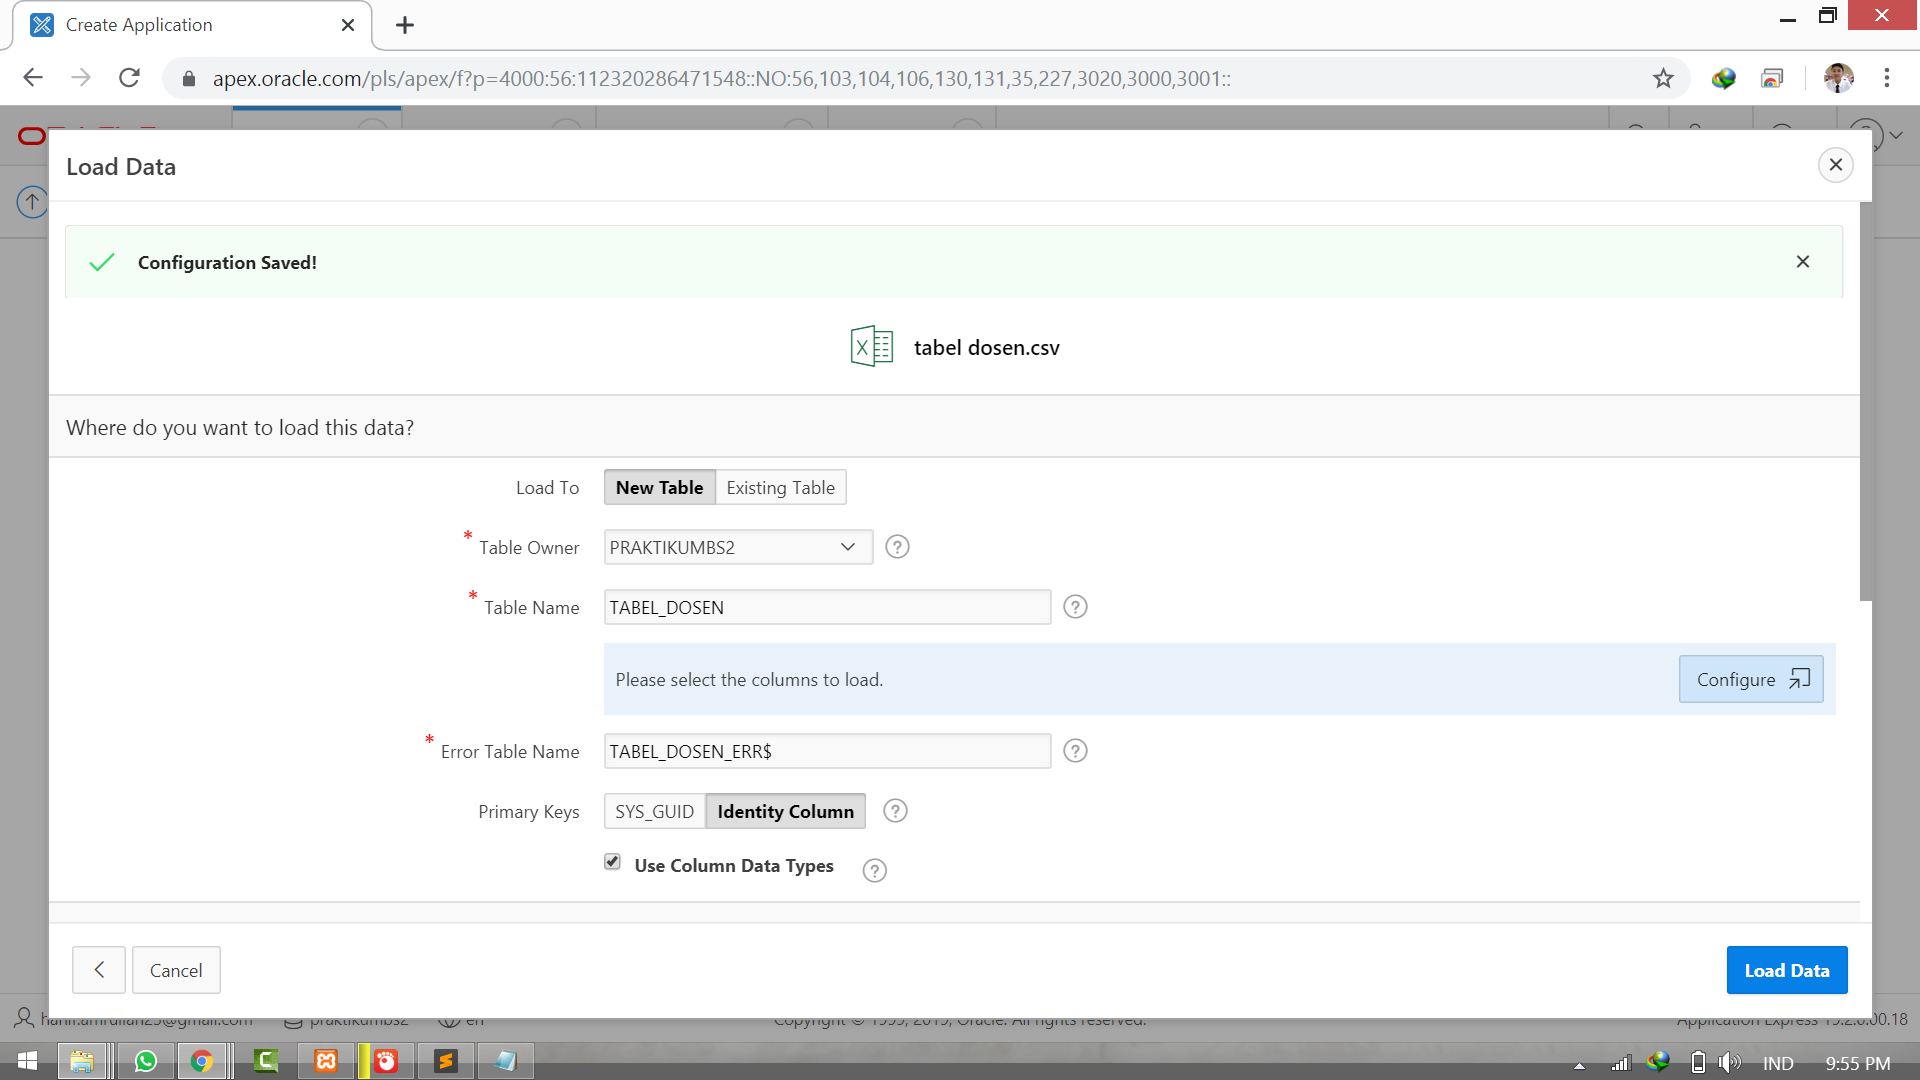
\includegraphics[scale=0.1]{img/8LoadDataTabel.png}}
        \caption{}
		\label{langkah9}
\end{figure}

\item ikuti
\begin{figure}
        \centerline{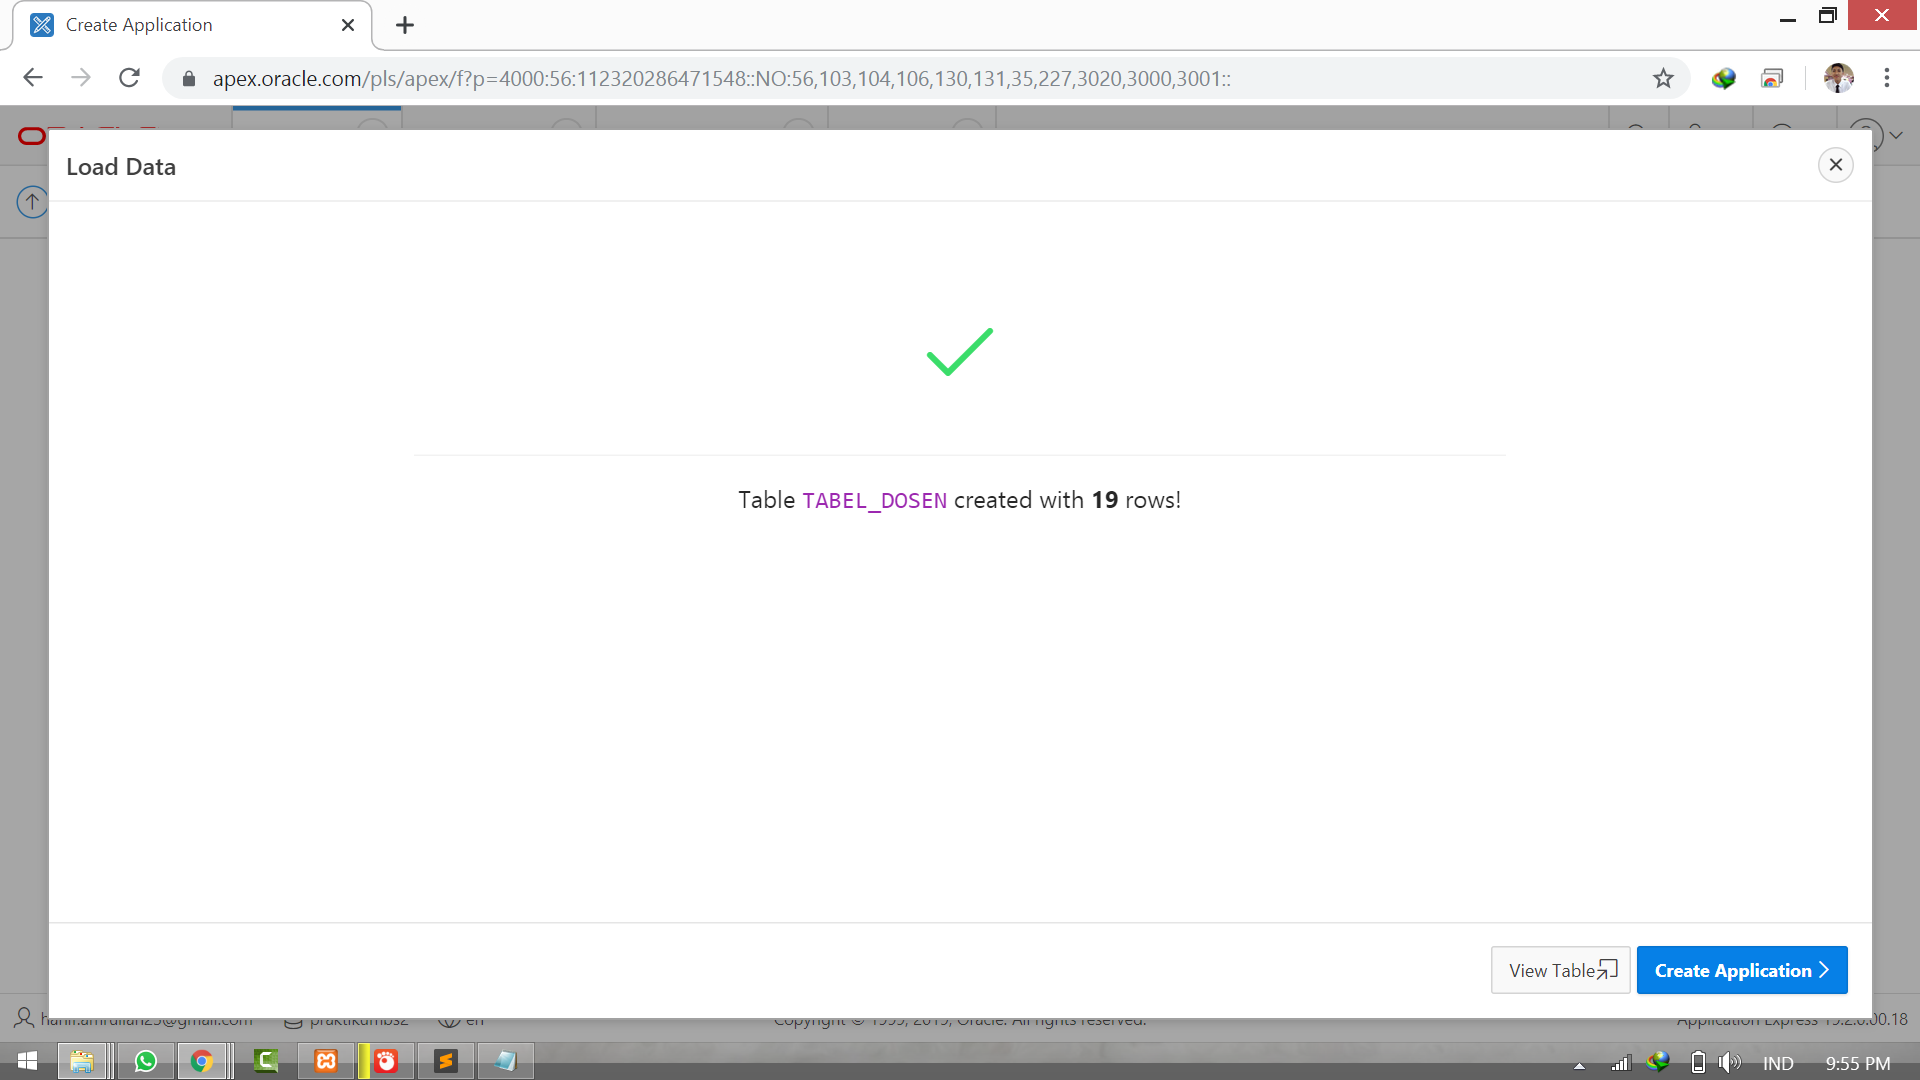
\includegraphics[scale=0.1]{img/9CreateTabel.png}}
        \caption{}
		\label{langkah10}
\end{figure}

\item ikuti
\begin{figure}
        \centerline{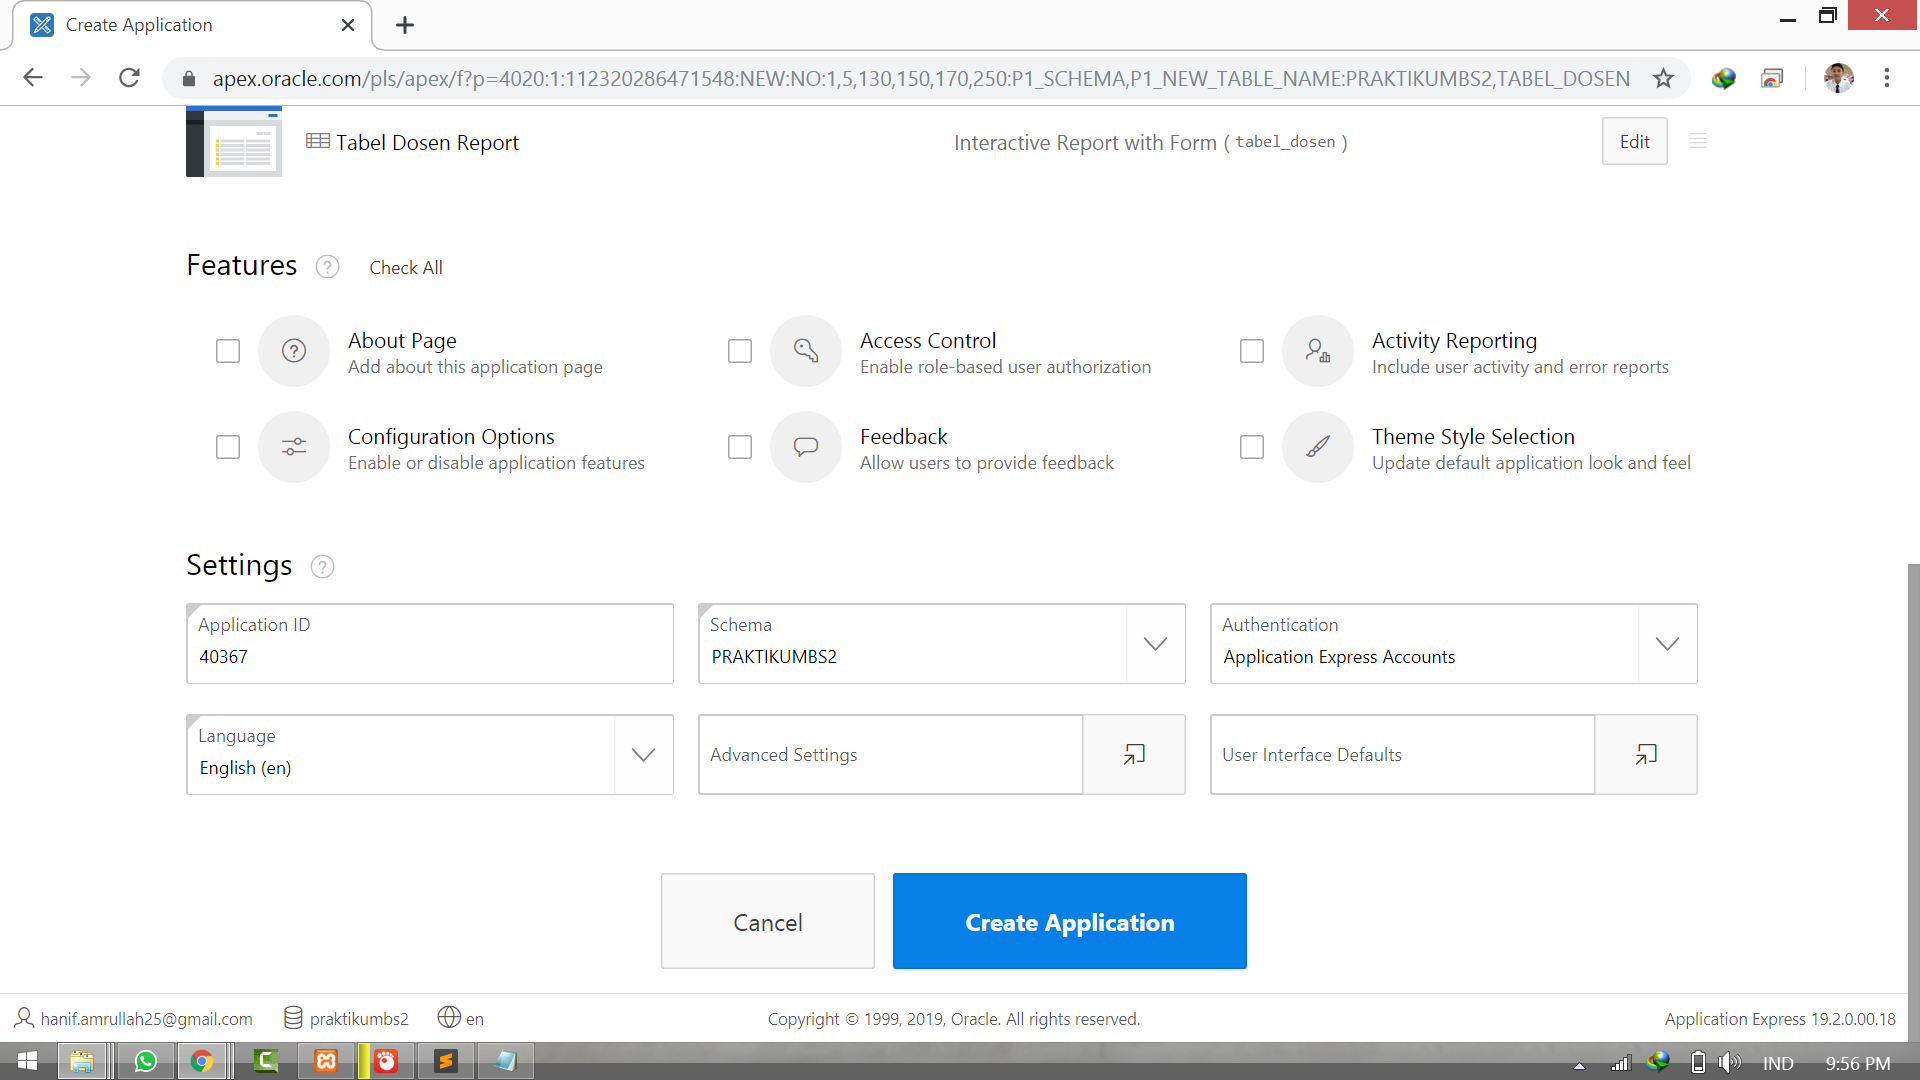
\includegraphics[scale=0.1]{img/10CreateTabel2.png}}
        \caption{}
		\label{langkah11}
\end{figure}

\item ikuti
\begin{figure}
        \centerline{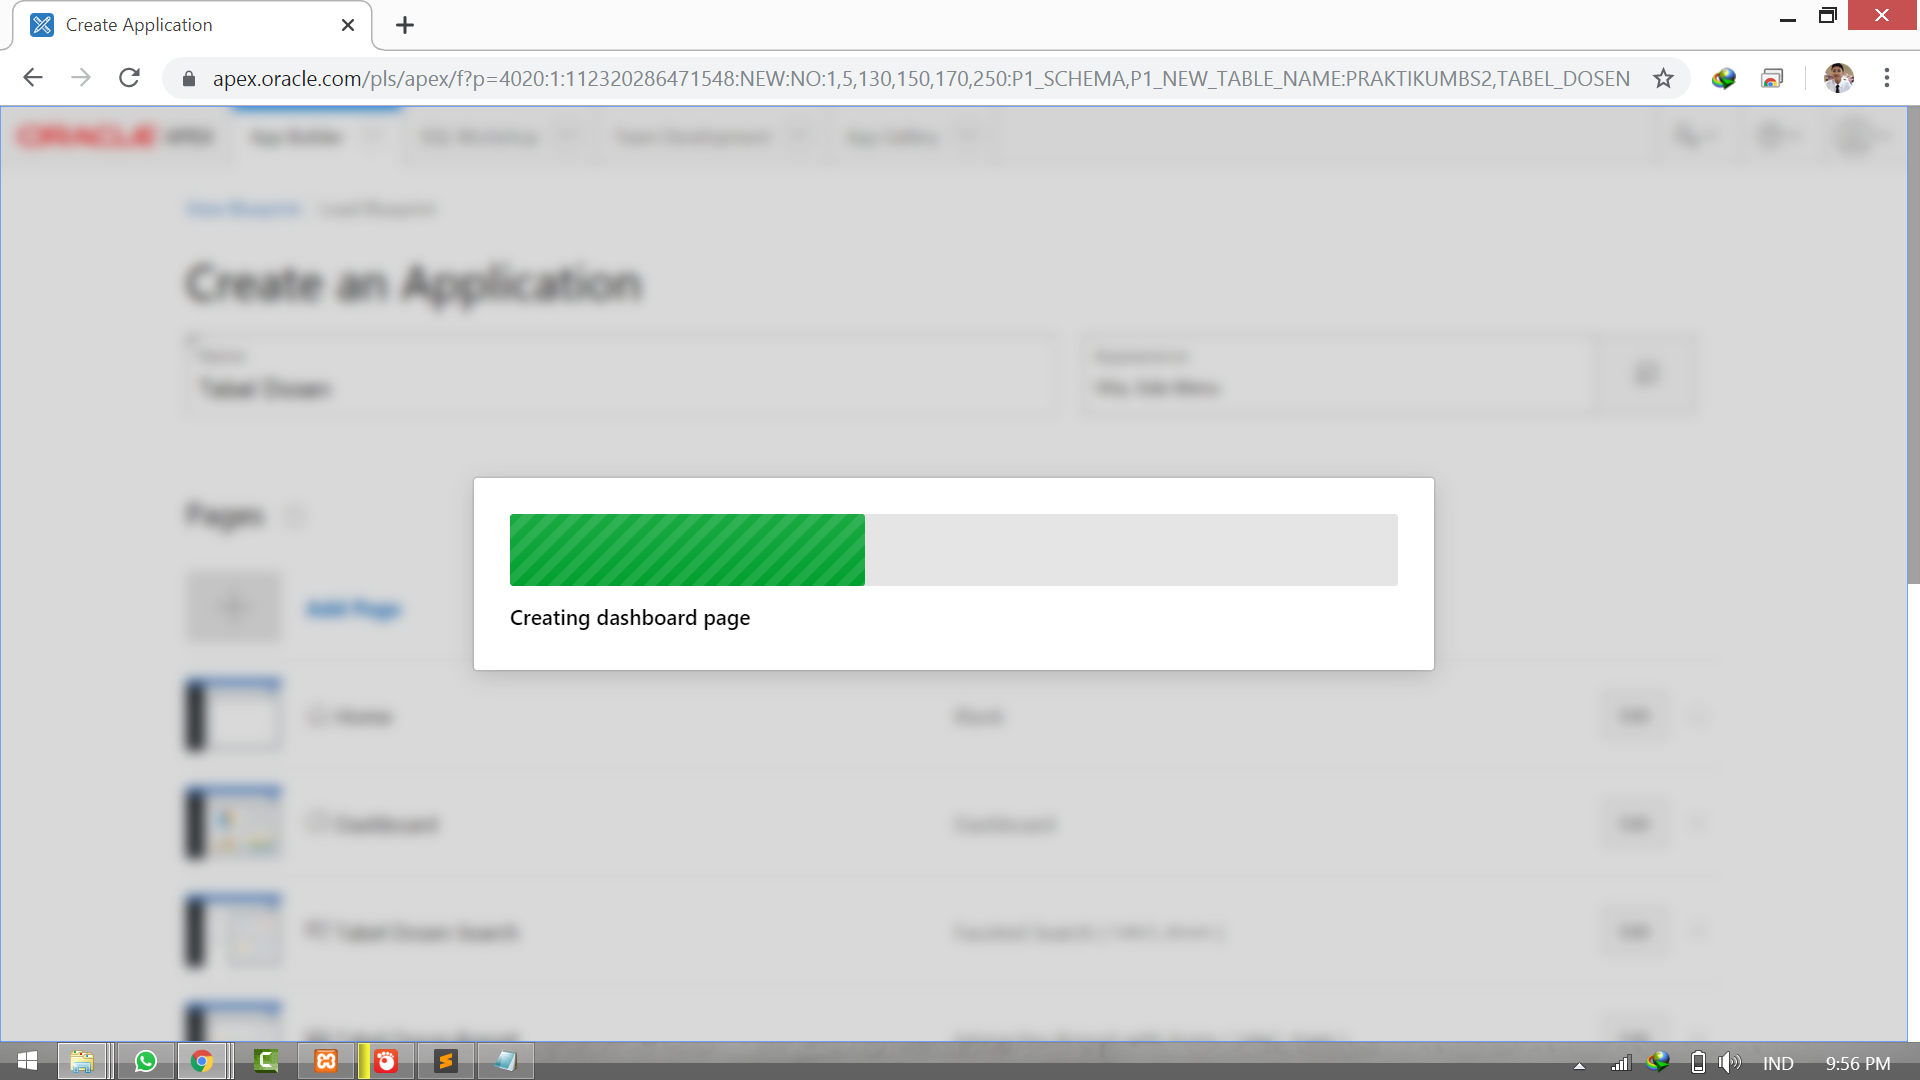
\includegraphics[scale=0.1]{img/11proses.png}}
        \caption{}
		\label{langkah12}
\end{figure}

\item ikuti
\begin{figure}
        \centerline{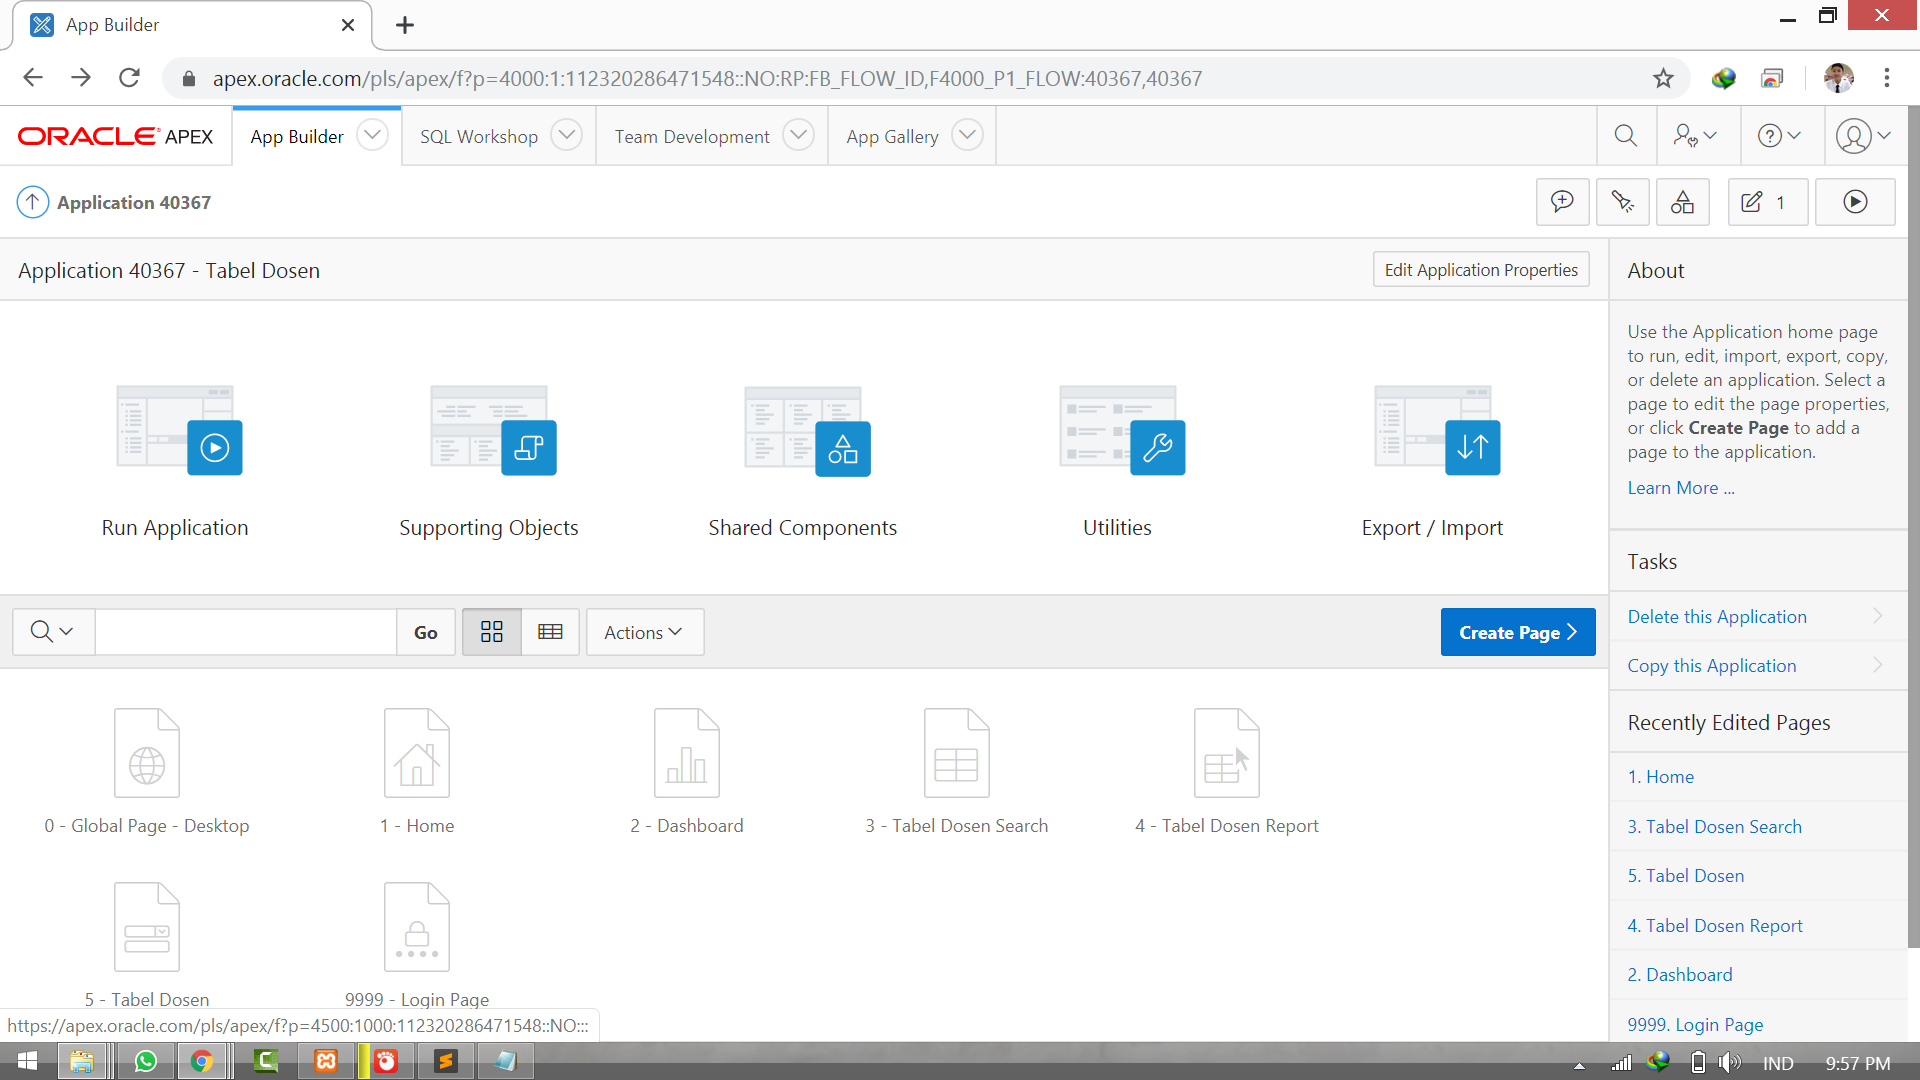
\includegraphics[scale=0.1]{img/12appbuilderlagi.png}}
        \caption{}
		\label{langkah13}
\end{figure}

\item ikuti
\begin{figure}
        \centerline{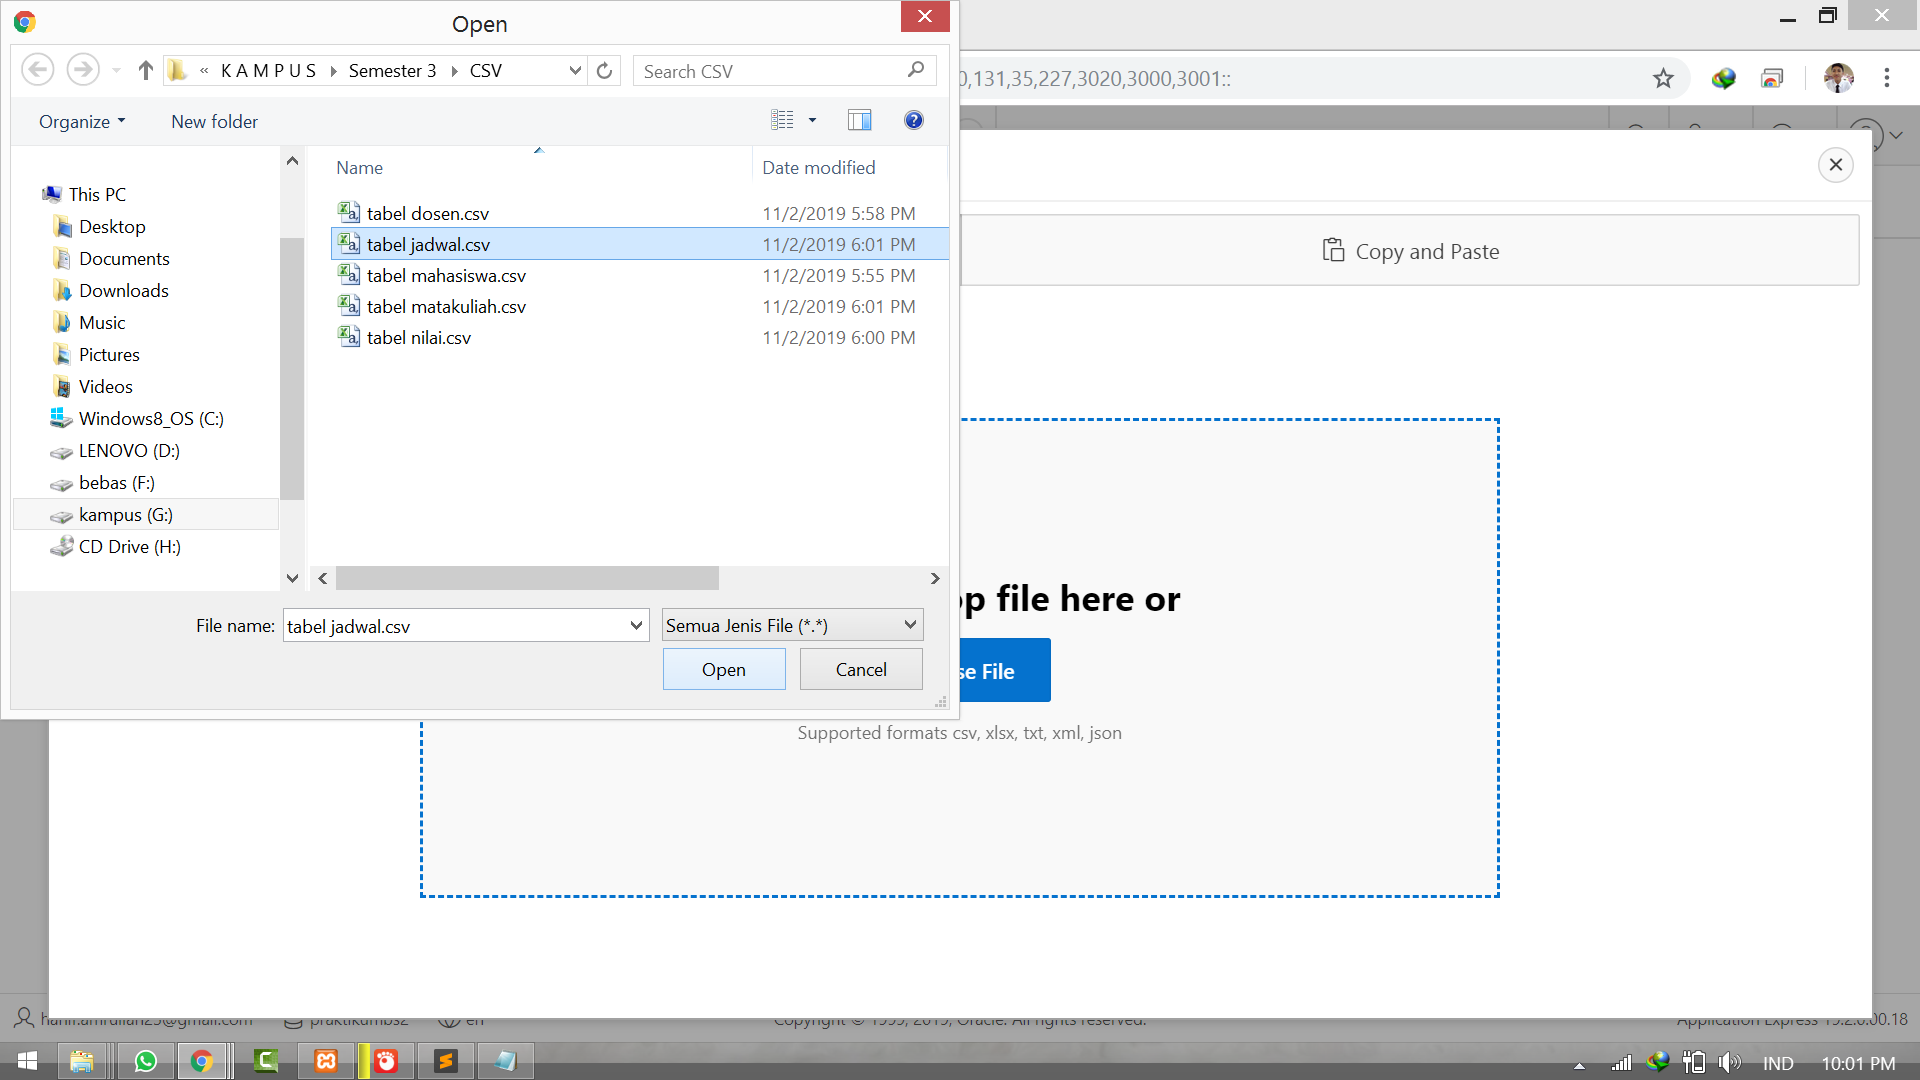
\includegraphics[scale=0.1]{img/13dragtabel.png}}
        \caption{}
		\label{langkah14}
\end{figure}

\item ikuti
\begin{figure}
        \centerline{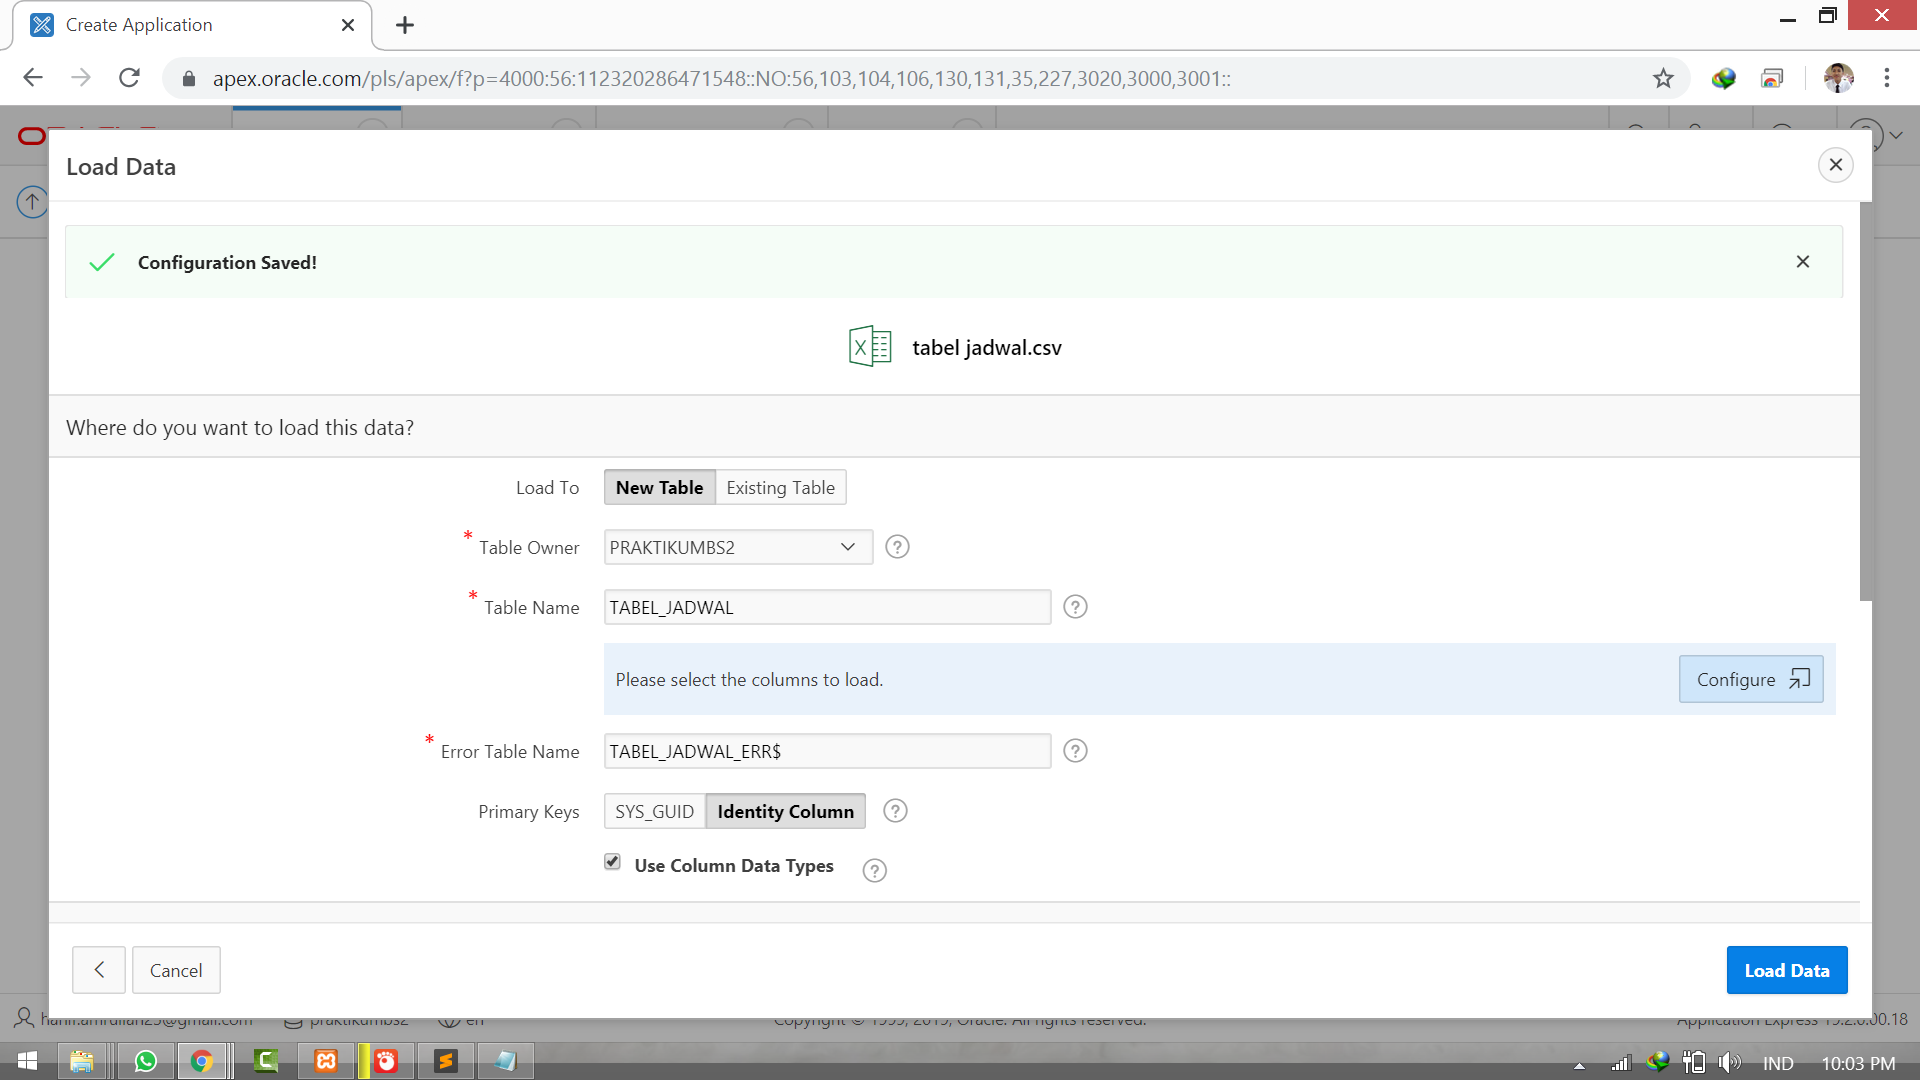
\includegraphics[scale=0.1]{img/14loaddatatabel.png}}
        \caption{}
		\label{langkah15}
\end{figure}

\item ikuti
\begin{figure}
        \centerline{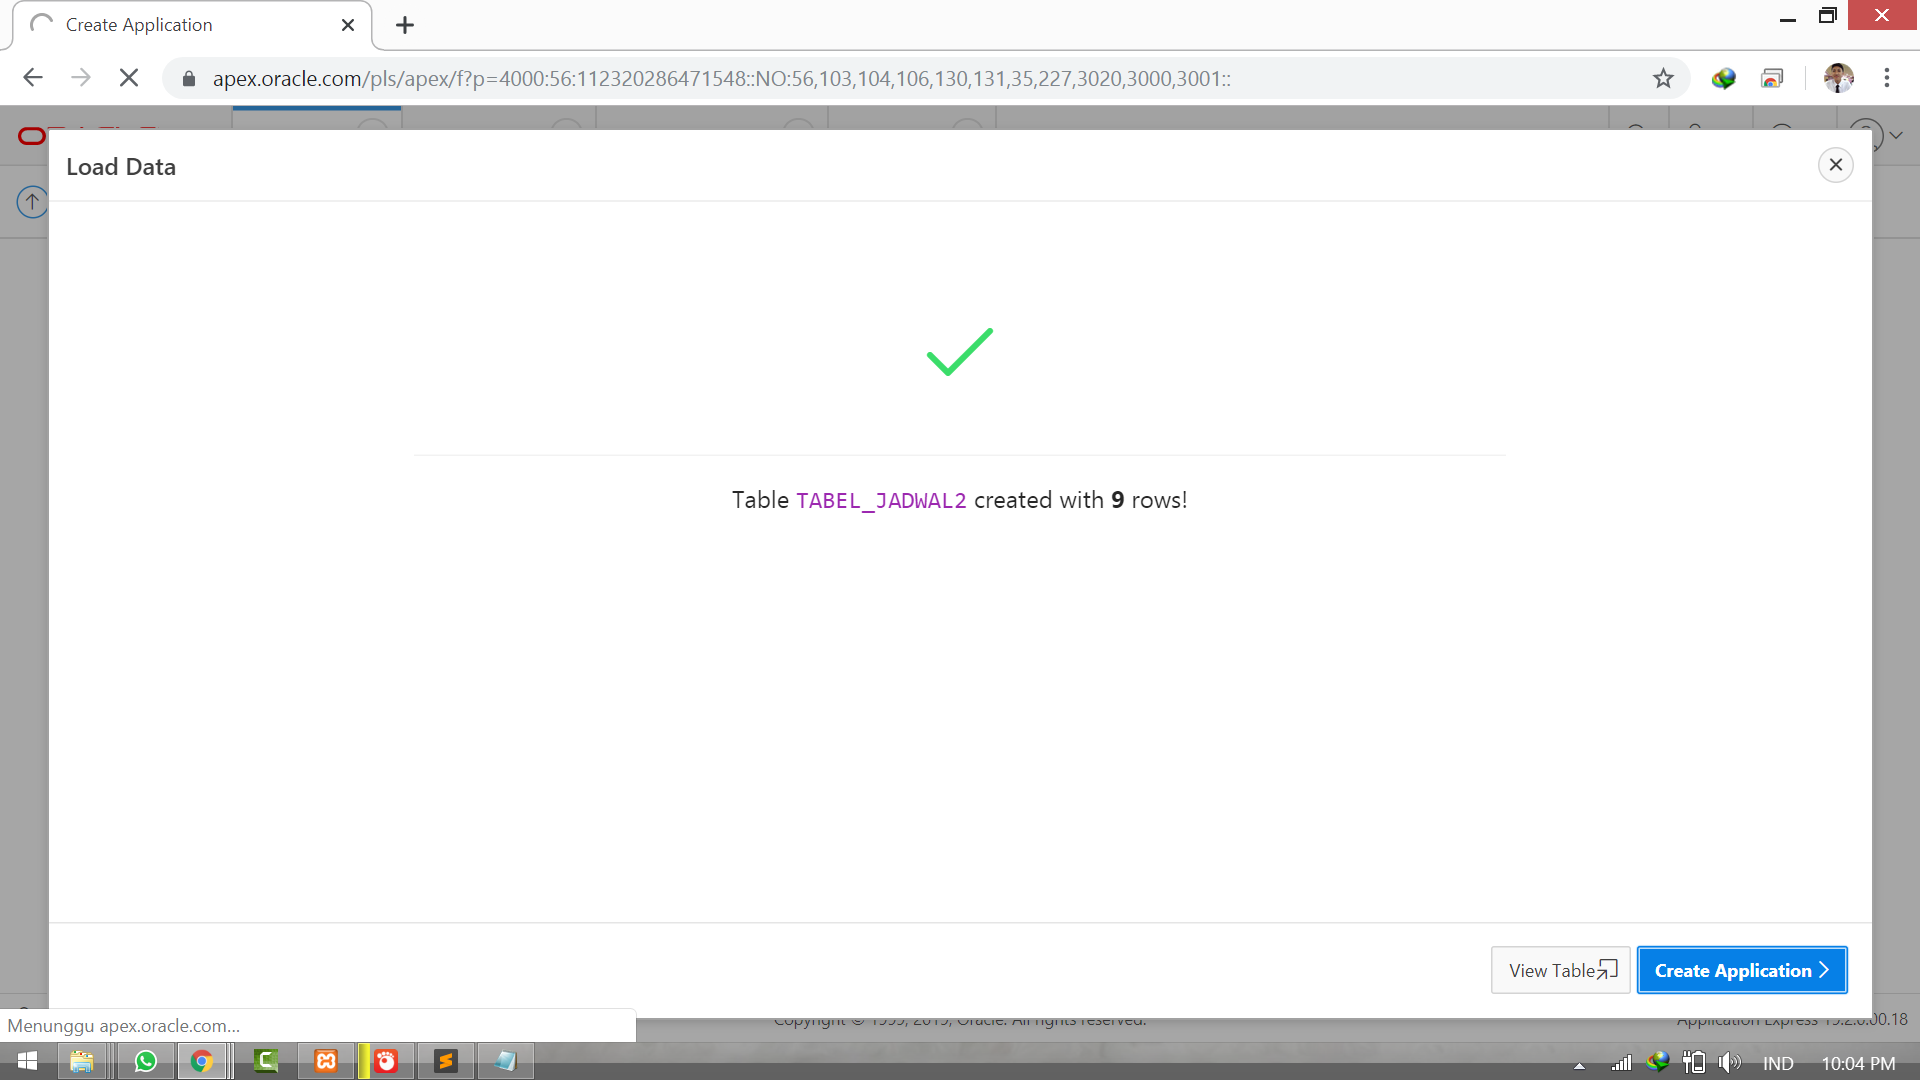
\includegraphics[scale=0.1]{img/15createtabel.png}}
        \caption{}
		\label{langkah16}
\end{figure}

\item ikuti
\begin{figure}
        \centerline{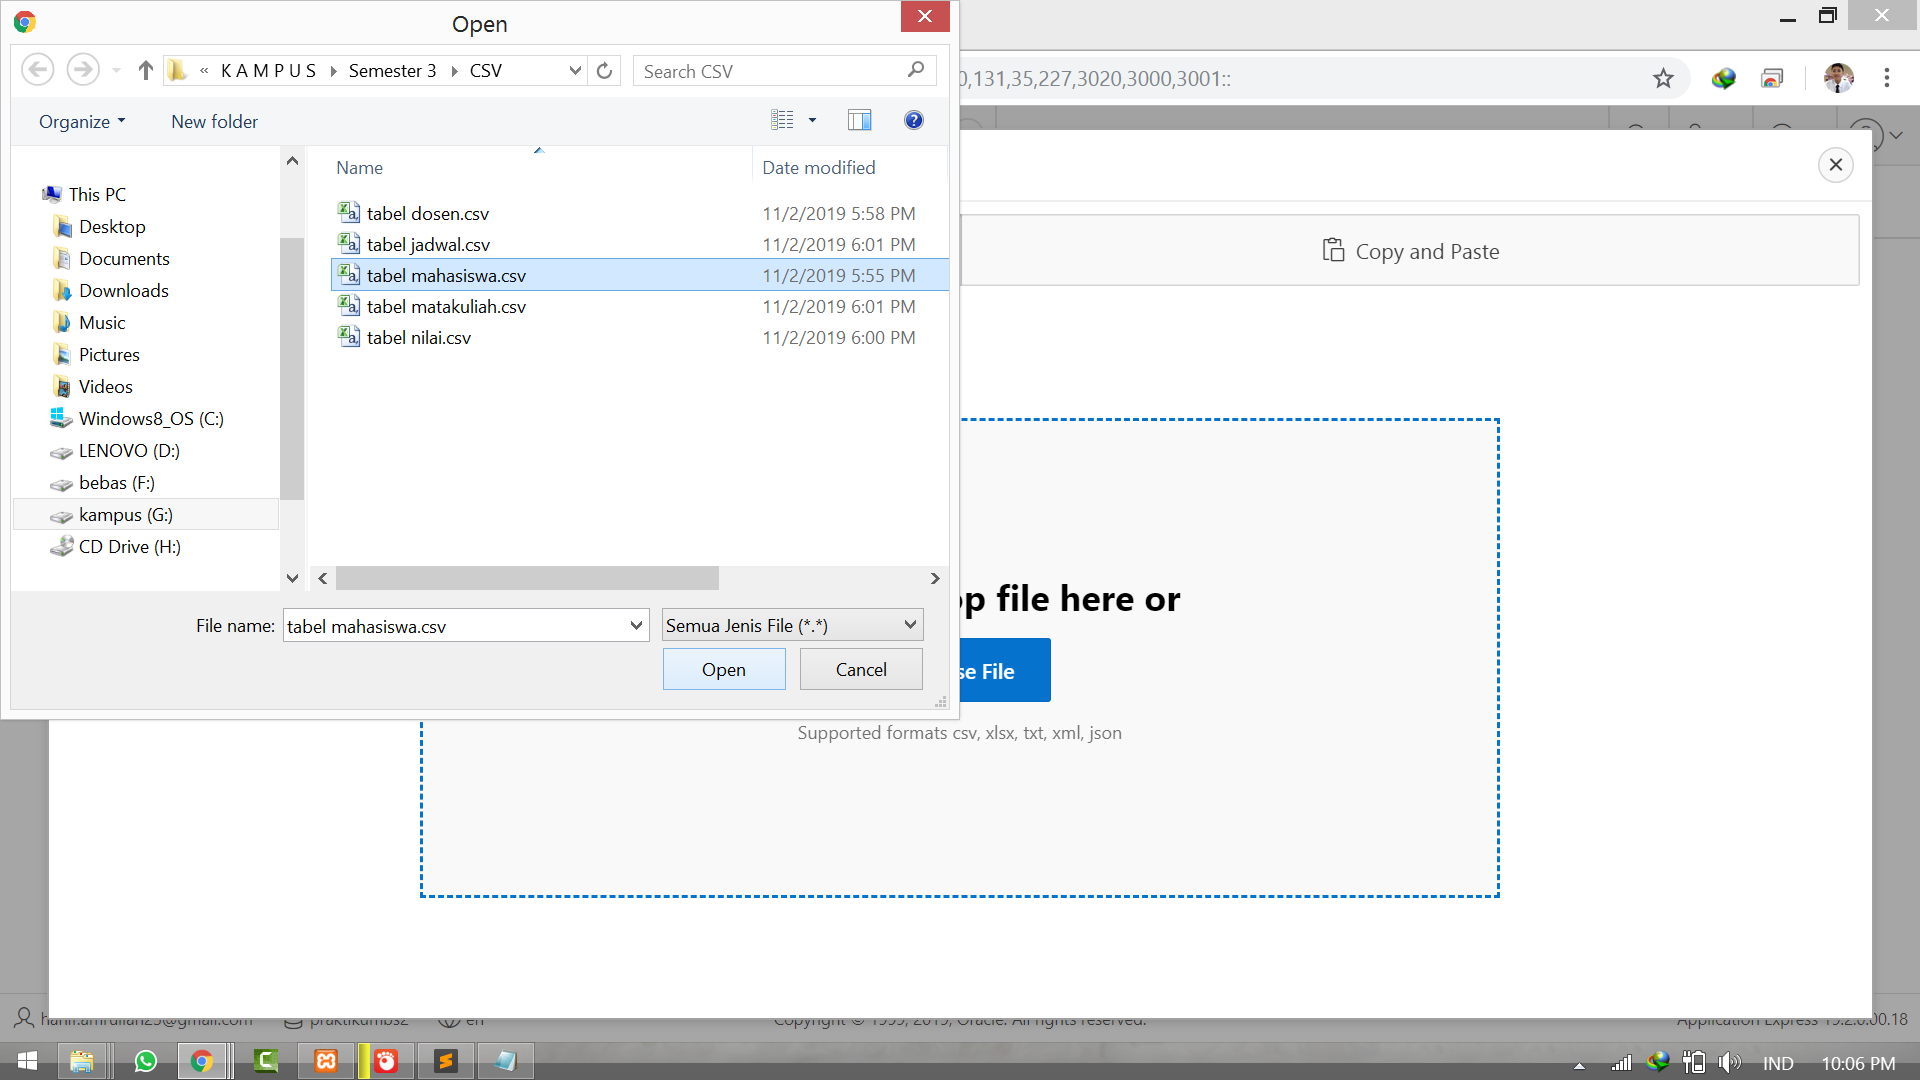
\includegraphics[scale=0.1]{img/16dragtabel.png}}
        \caption{}
		\label{langkah17}
\end{figure}

\item ikuti
\begin{figure}
        \centerline{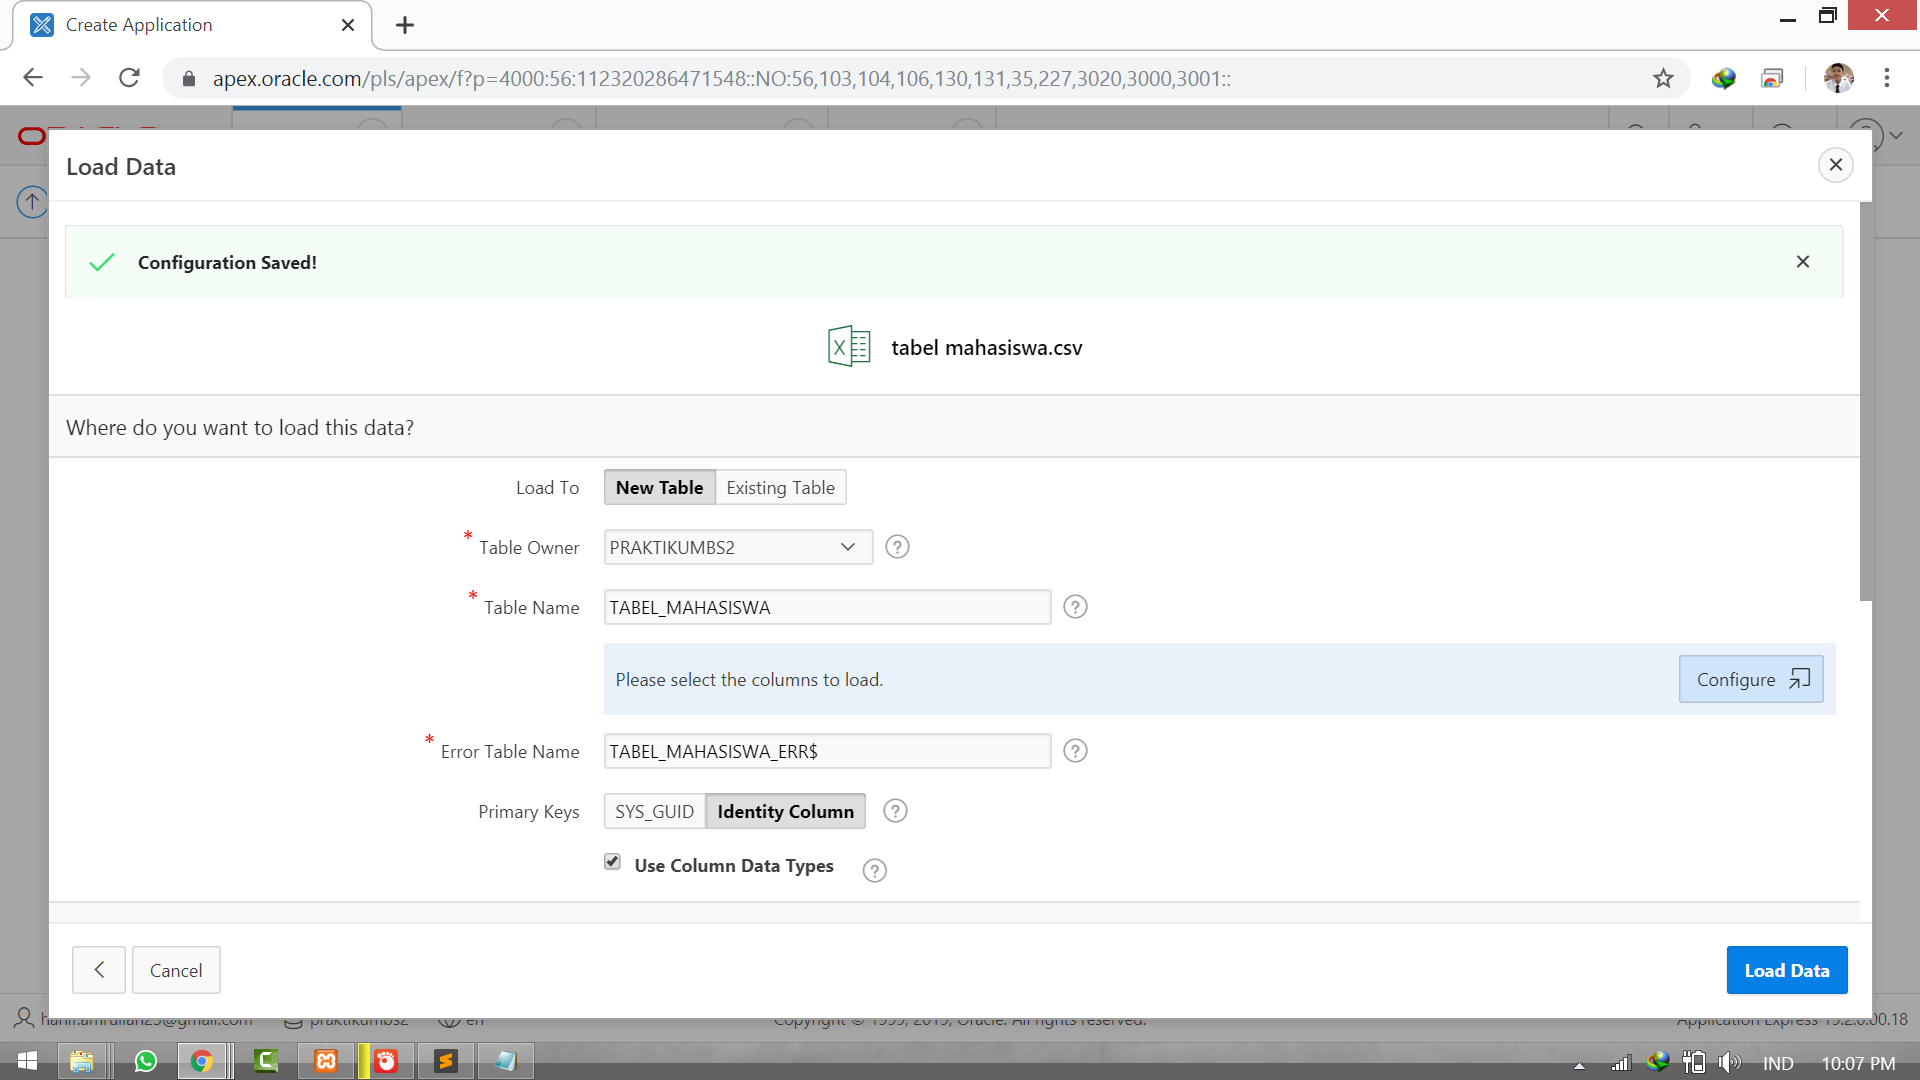
\includegraphics[scale=0.1]{img/17loaddatatetabel.png}}
        \caption{}
		\label{langkah18}
\end{figure}

\item ikuti
\begin{figure}
        \centerline{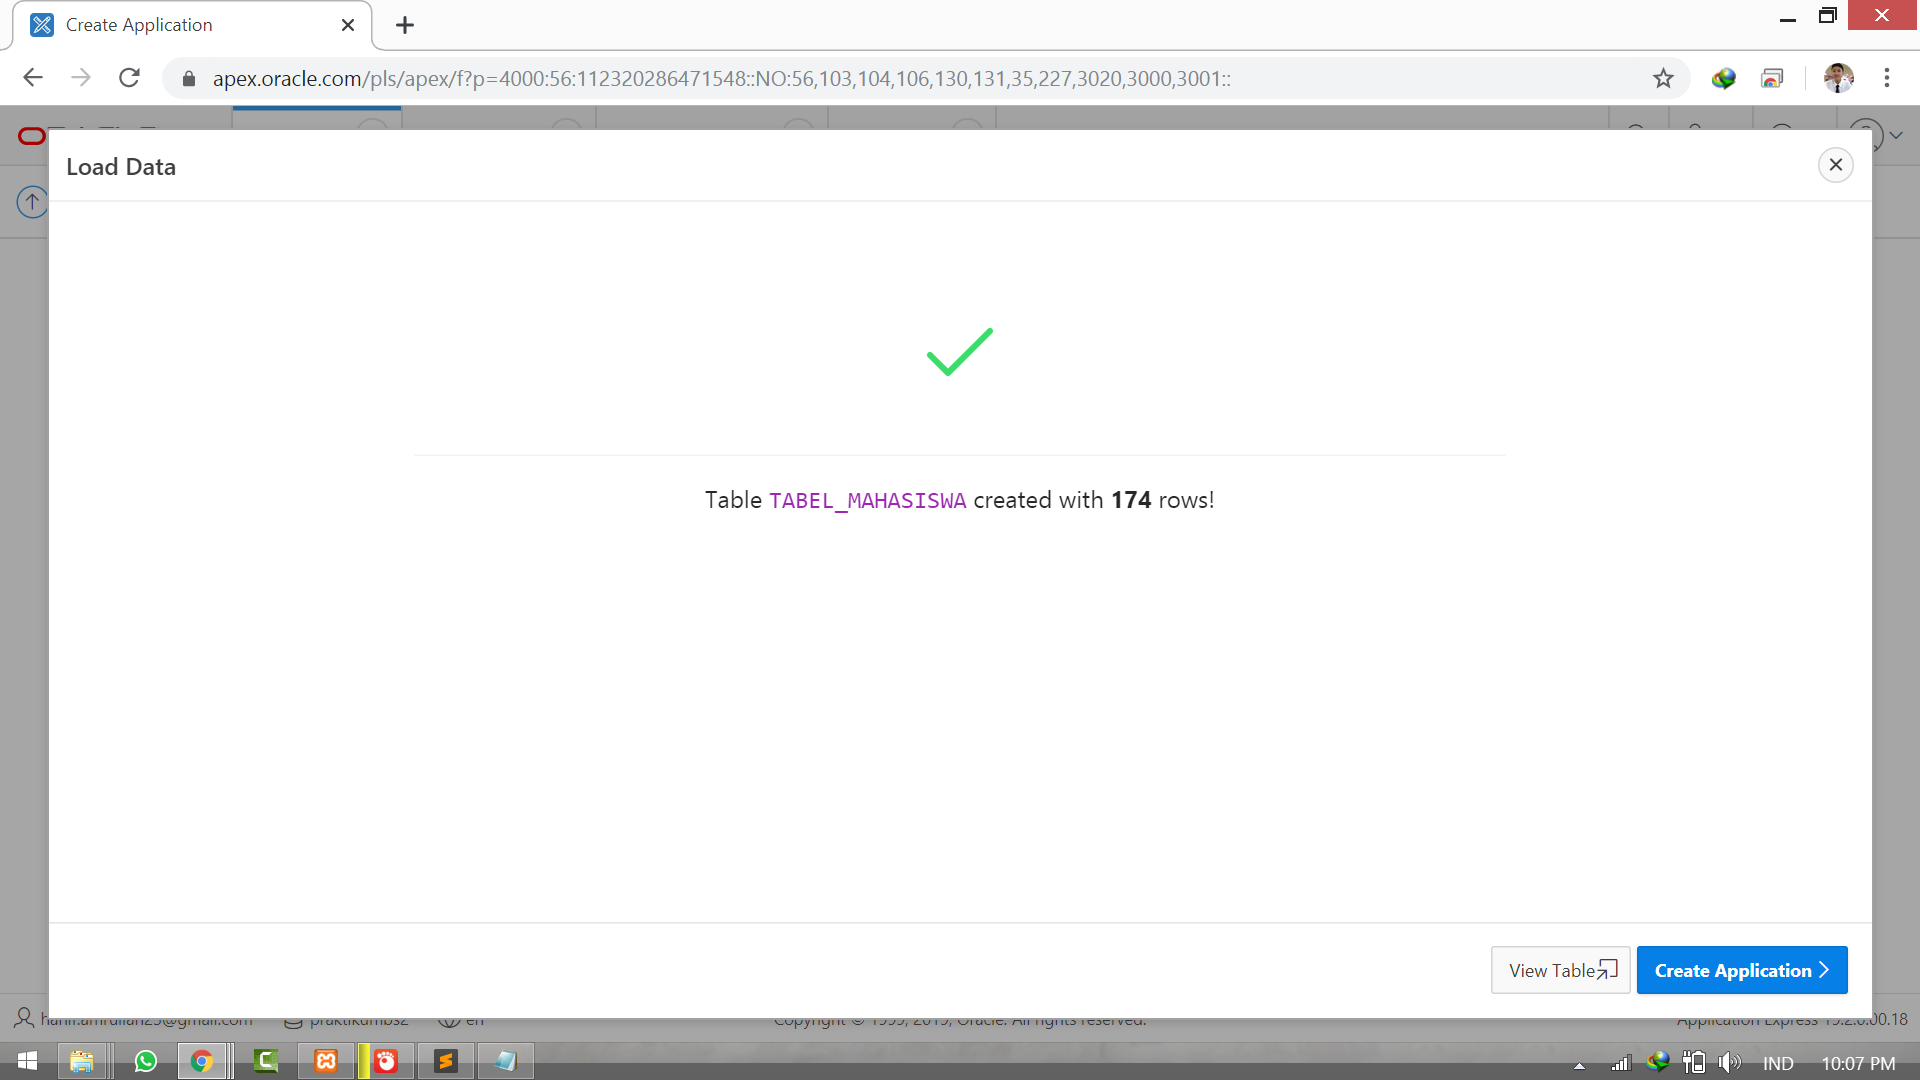
\includegraphics[scale=0.1]{img/18createtabel.png}}
        \caption{}
		\label{langkah19}
\end{figure}

\item ikuti
\begin{figure}
        \centerline{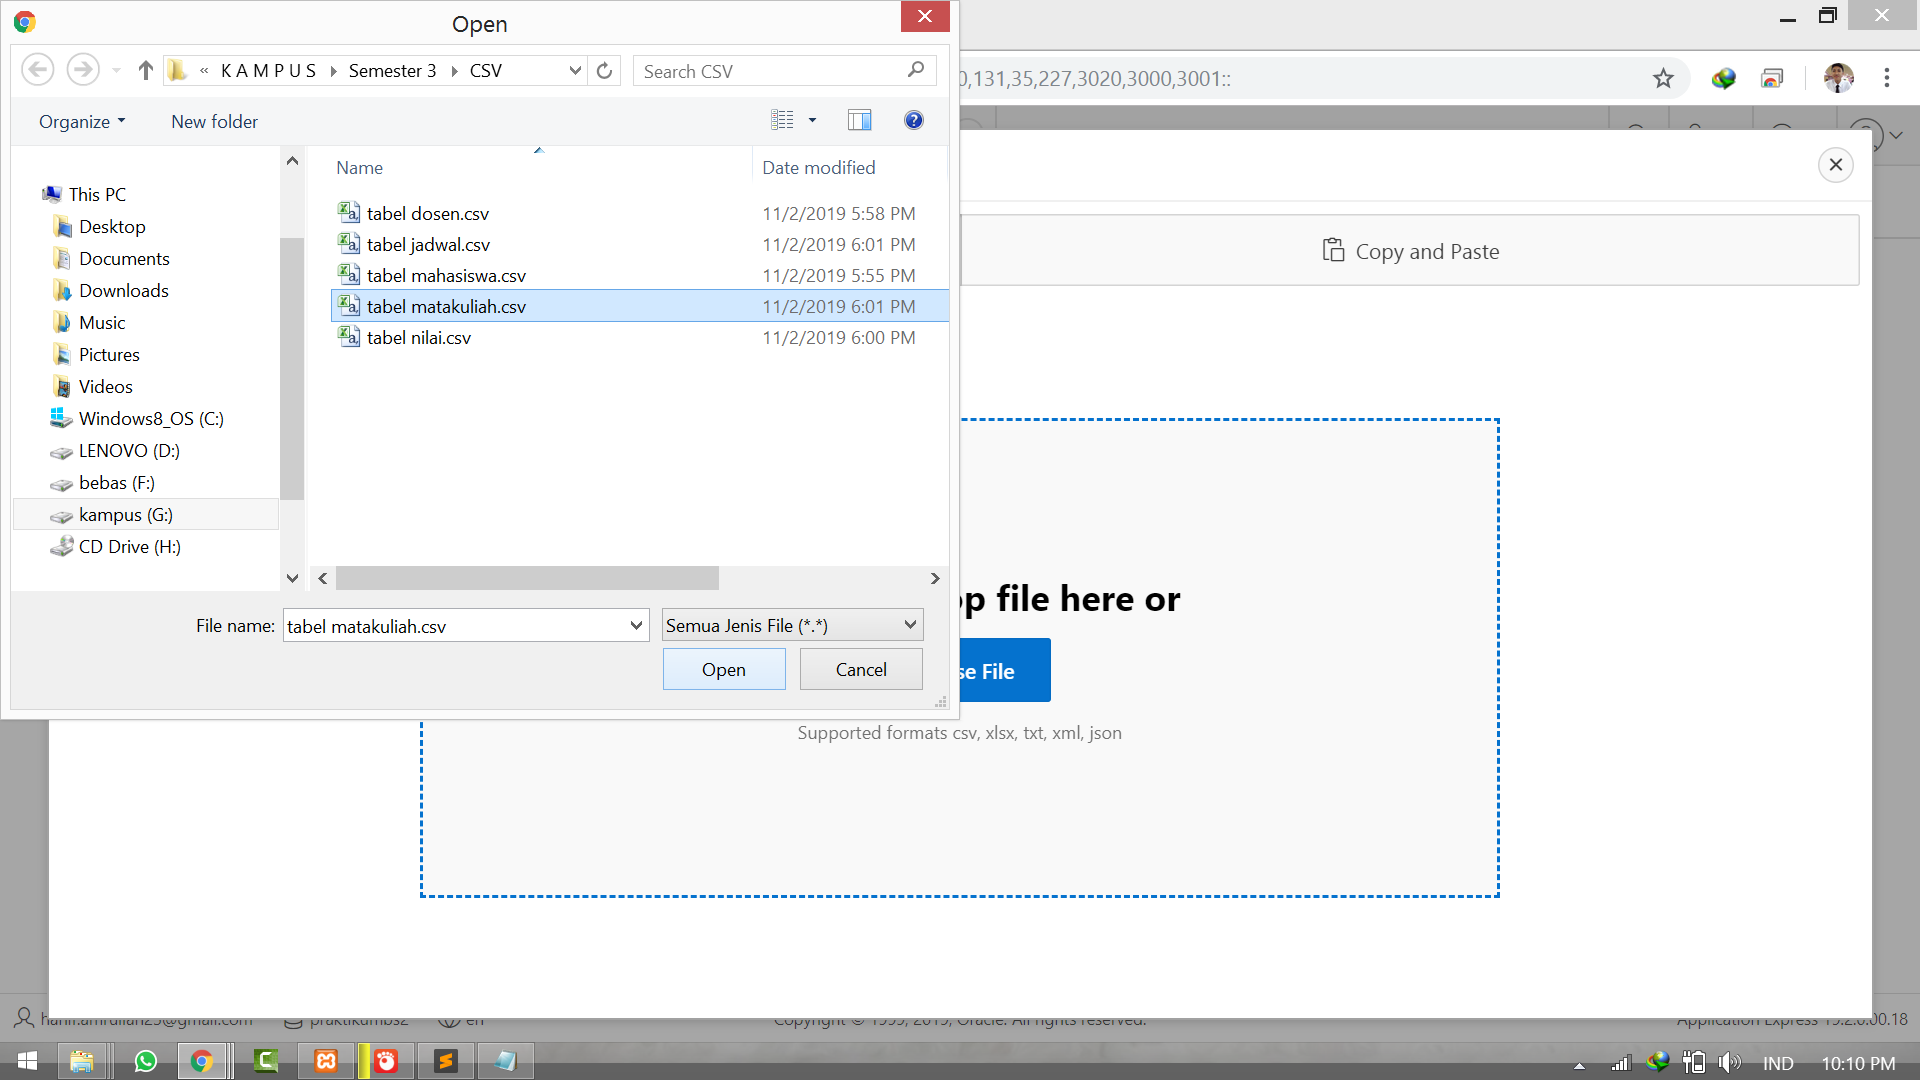
\includegraphics[scale=0.1]{img/19dragtabel.png}}
        \caption{}
		\label{langkah20}
\end{figure}

\item ikuti
\begin{figure}
        \centerline{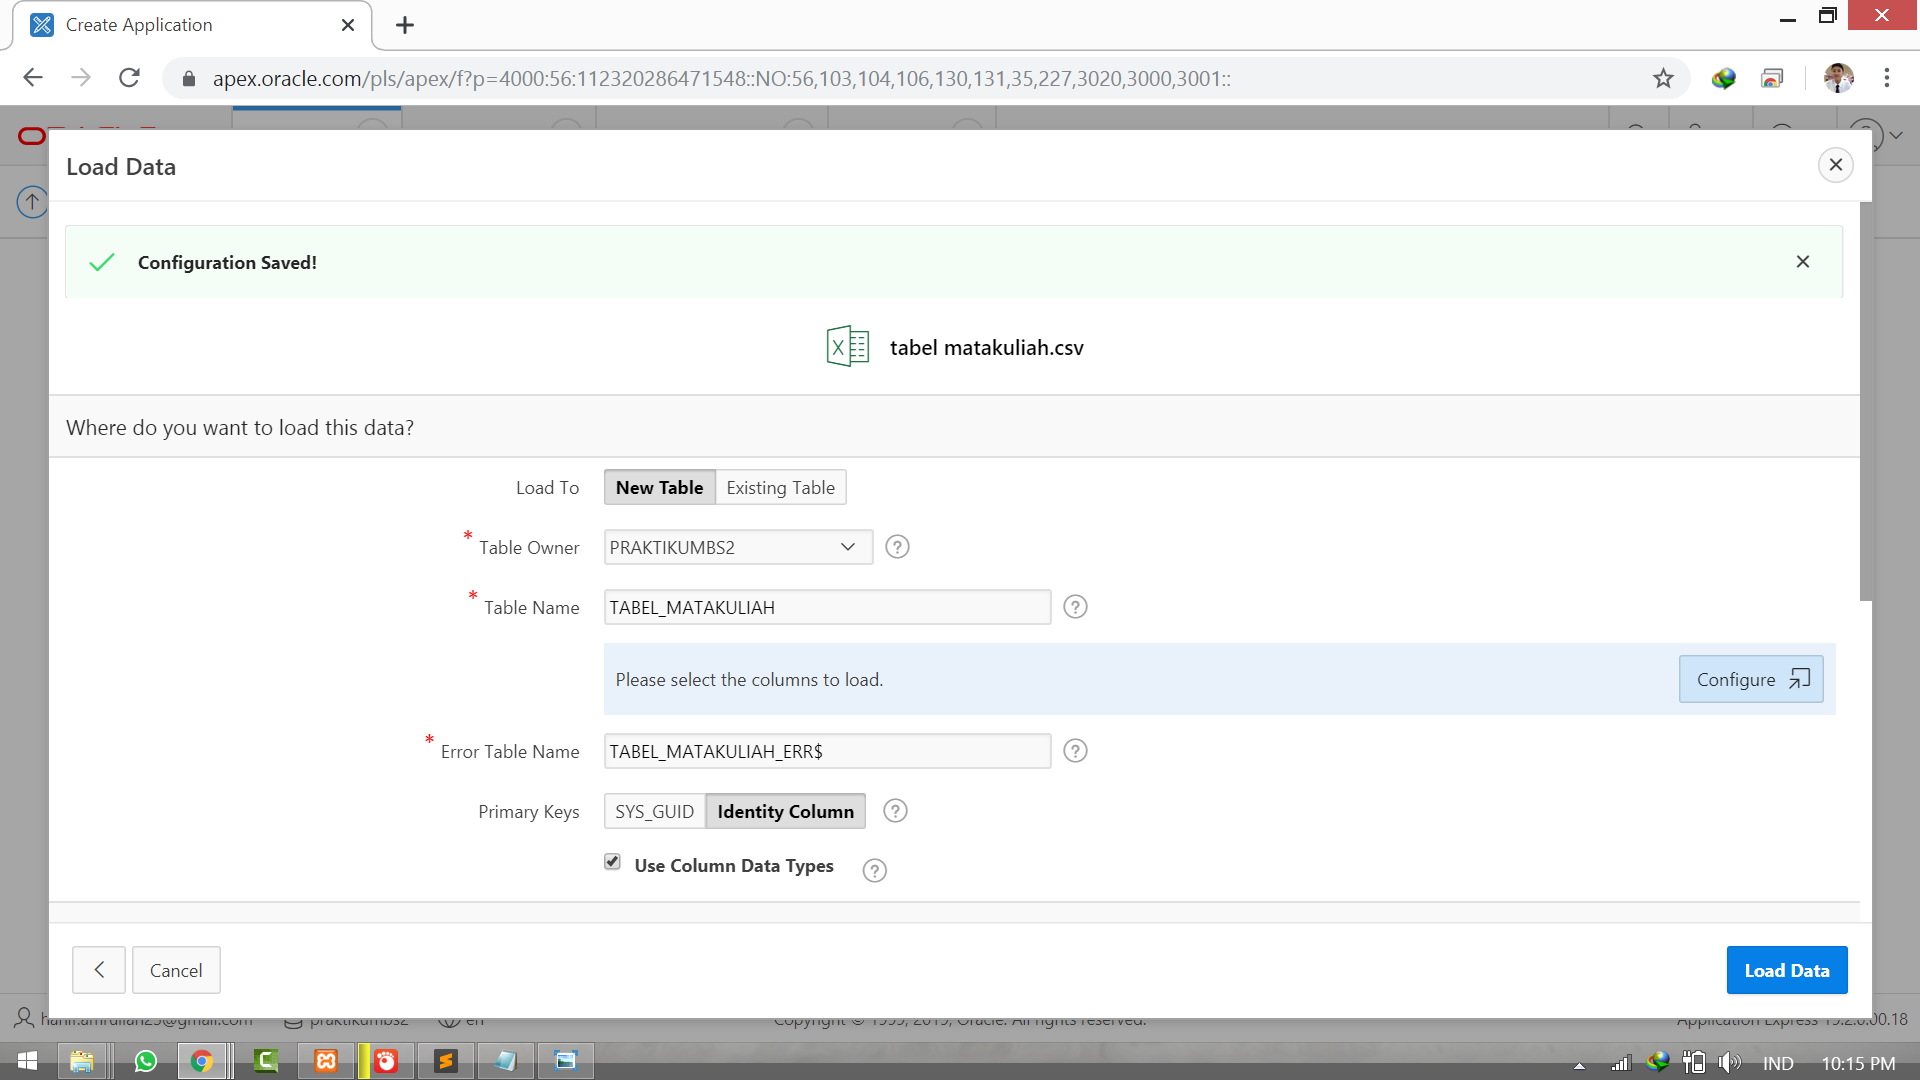
\includegraphics[scale=0.1]{img/20loaddatatabel.png}}
        \caption{}
		\label{langkah21}
\end{figure}

\item ikuti
\begin{figure}
        \centerline{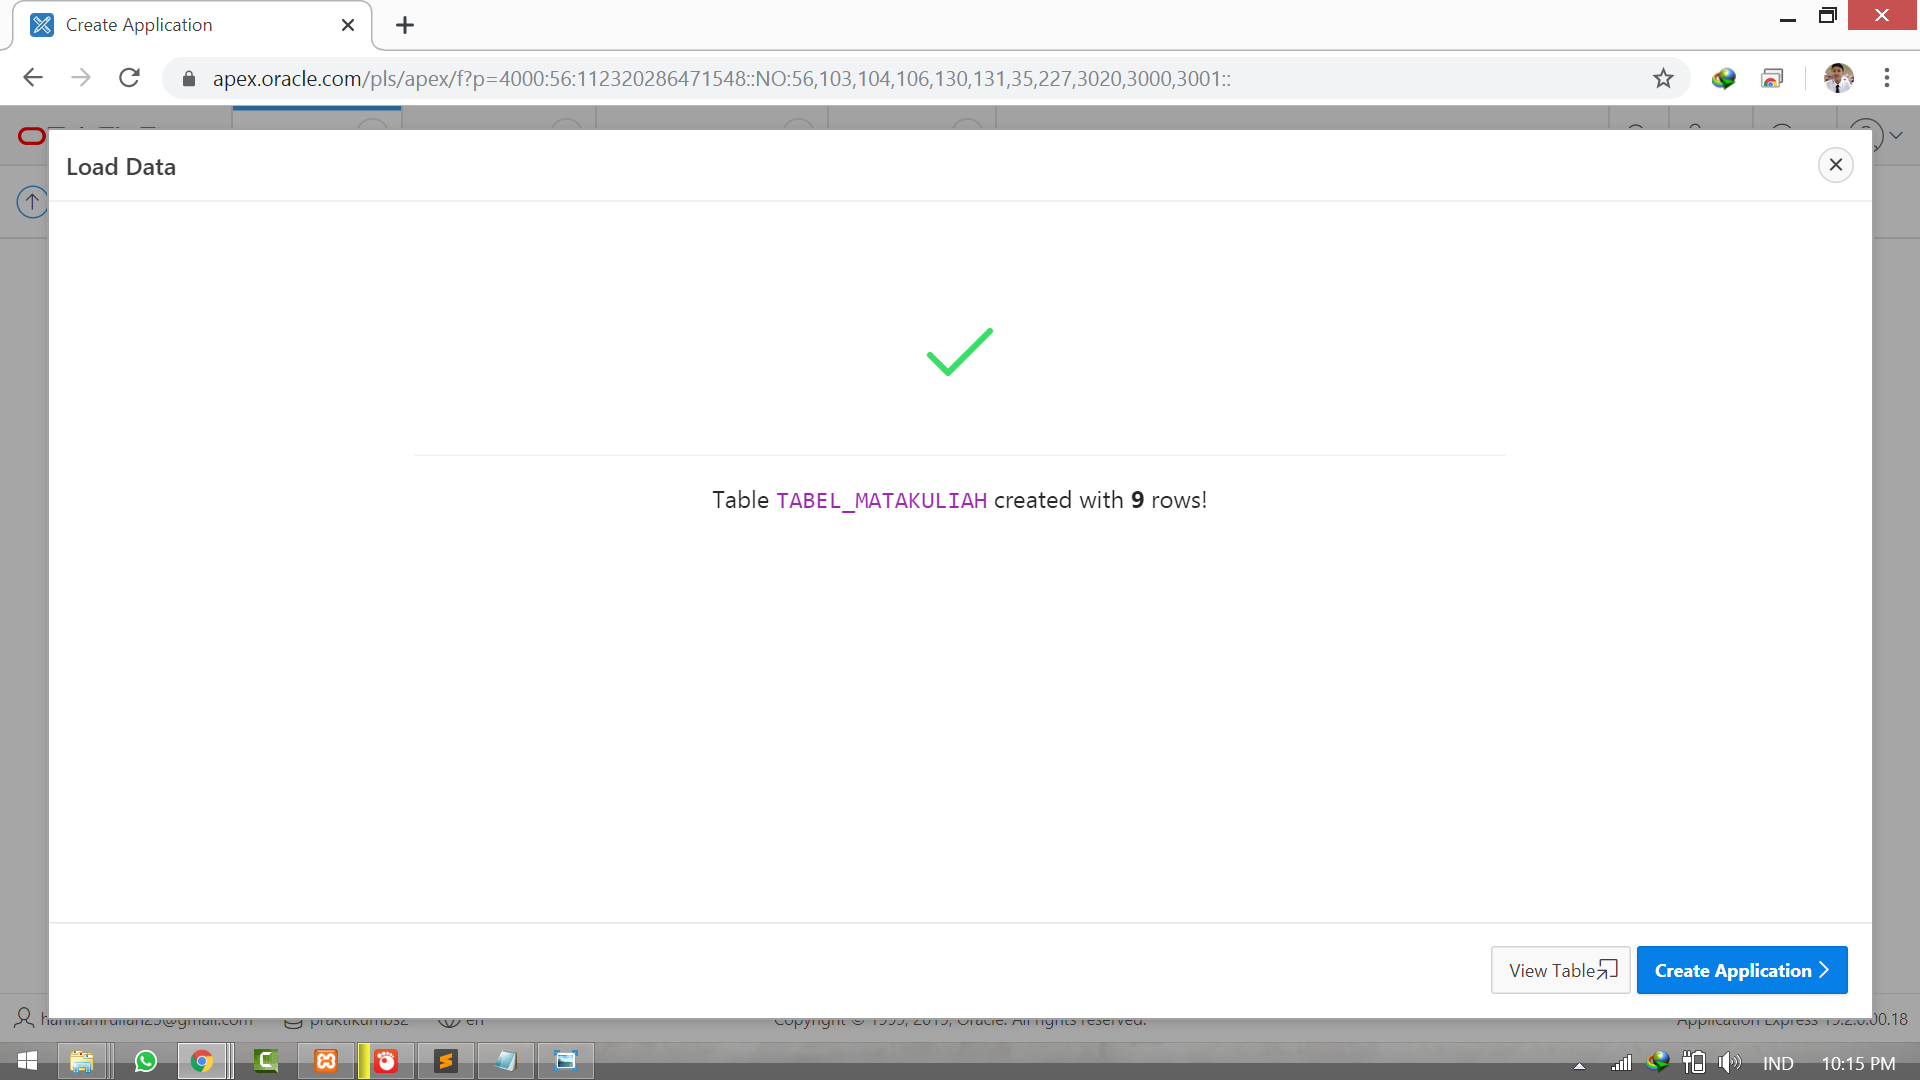
\includegraphics[scale=0.1]{img/21createtabel.png}}
        \caption{}
		\label{langkah22}
\end{figure}
	\end{enumerate}
	
\newpage	
user: hanif.amrullah25@gmail.com\\
password:zxasqw12\\
Link:https://apex.oracle.com/pls/apex/f?p=81839:1:1138517272936:::::\\
\end{document}
